\chapter{Analysis of the spread of news on Twitter and traditional media}

%%%%%%%%%%%%%%%%%%%%%%%%%%%%%%%%%%%%%%%%%%%%%%%%%%%%%%%%%%%%%%%%
%%%%%%%%%%%%%%%%%%%%%%%%%%%%%%%%%%%%%%%%%%%%%%%%%%%%%%%%%%%%%%%%
\section{Introduction\label{Sec:Introduction}}
%%%%%%%%%%%%%%%%%%%%%%%%%%%%%%%%%%%%%%%%%%%%%%%%%%%%%%%%%%%%%%%%
%%%%%%%%%%%%%%%%%%%%%%%%%%%%%%%%%%%%%%%%%%%%%%%%%%%%%%%%%%%%%%%%

Nearly three fourth of the American adults use social media, and more than two-thirds report that they get at least some of their news on them \citep{Pew2018_SocialMediaFactSheet,Pew2019_MobileTechnololy}. While there is growing concern about misinformation online and the consumption of fake news \citep{AllcottGentzkow2017,AllcottGentzkowYu2019_ReasearchPolitics}, little is known on the impact social media have on the production of news. Yet, not only social media affect the way we consume news, but also the way news is produced, including by traditional media. First, social media users may report events before traditional media \citep{Sakakietal2010}.\footnote{As highlighted by Alan Rusbridger as soon as 2010, \textit{``increasingly, news happens first on Twitter."} (...) \textit{``If you're a regular Twitter user, even if you're in the news business and have access to wires, the chances are that you'll check out many rumours of breaking news on Twitter first. There are millions of human monitors out there who will pick up on the smallest things and who have the same instincts as the agencies — to be the first with the news. As more people join, the better it will get."} Source: https://www.theguardian.com/media/2010/nov/19/alan-rusbridger-twitter.} Second, news editors may use social media as a signal to draw inferences about consumers' preferences. Further, social media compete with mainstream media for consumer's attention, and this may affect publishers' incentives to invest in quality \citep{deCorniereSarvary2019}.

In this article, we investigate how editors decide on the coverage for stories, and in particular the role played by social media in their decision. To do so, we have built a completely new dataset including around $70\%$ of all the tweets in French during one year (July 2018 - July 2019) and the content produced online by the French-speaking general information media outlets during the same time period ($205$ media included, independently of their offline format\footnote{Our dataset includes all the content published online by French general information newspapers, TV channels, radio stations, pure online media, and the news agency AFP as well as the content produced online by $10$ French-speaking foreign media outlets such as \textit{Le Temps} (Switzerland). More details on the data collection are provided in Section \ref{Sec:DataNews}).} Our dataset contains around $1.8$ billion tweets as well as $4$ million news articles. For each tweet (that can be original tweets but also retweets or quotes of past tweets) as well as each news article, we determine their precise ``publication" time. Furthermore, we collect information on the Twitter users, in particular their number of followers and the number of interactions generated by their tweets.

First, we develop a new detection algorithm to identify news events on Twitter -- the social media events or SME henceforth -- together with an algorithm to identify news events on mainstream media -- mainstream media events or MME henceforth. Second, we develop ``community detection" algorithms to investigate the relationship between SMEs and MMEs. When an event is covered both on social and on mainstream media, we determine where the information originates. For the subset of events that originates first on social media, we study whether the event popularity on Twitter impacts the coverage mainstream media devote to this event.

The scale of our dataset (one year of data with several millions of tweets and of news articles) allows us to follow a split-sample approach to relieve concerns about specification search and publication bias \citep{Leamer1978,Leamer1983,Glaeser2006_incentives}.\footnote{We thank Jesse Shapiro for suggesting us this approach.} Following \citet{FafchampsLabonne2016,FafchampsLabonne2017} and \citet{AndersonMagruder2017}, we first perform our analysis on the July 2018-September 2018 time period (three months of data). The results of this draft relies on this sub-sample that we use to narrow down the list of hypotheses we wish to test and to specify the research plan that we will pre-register. The final version of the paper will follow the pre-registered plan and perform the empirical analysis on the remainder of the data (October 2018-July 2019).

The sample we use in this version of the article to delineate our research plan (July 2018-September 2018) includes $428$ million tweets and $929,764$ news articles. We identify $5,766$ joint events. Producing these data is our first contribution. It is to the best of our knowledge the most exhaustive dataset on social media and mainstream media events available to researchers. We think the algorithms we develop to analyze these data could also be of future use to other researchers studying online information. Our second contribution is descriptive. While there is a growing literature that studies the propagation of fake news on social media \citep{Vosoughietal2017,VosoughiRoyAral2018}, little is known on the propagation of information between social media and traditional media outlets. Besides, while false news only represent a small part of the news we consume, not much is known on the propagation of real information. In this article, we investigate the propagation of both real and false news between social and mainstream media.

Third and most importantly, we open the black box of newsroom production decisions, and investigate the extent to which news editors are influenced in their editorial decisions by stories popularity on social media. Focusing on the subset of news stories that originate first on Twitter ($4,259$ of of the $5,766$ joint events), we investigate how their popularity affects the coverage traditional media devote to these stories. The popularity of a story on Twitter is measured before the first news article devoted to the story; we use the total number of tweets related to the event, and the popularity of these tweets. We call the news breaker on Twitter the seed of the event.

The main empirical challenge here comes from the fact that a story popularity on Twitter and its media coverage can both be driven by the intrinsic interest of the story, independently of what happens on social media. Hence, to identify the specific role played by social media, we need to find exogenous sources of variation of a story popularity on Twitter. To do so, we propose a new instrument that relies on the interaction between the structure of the Twitter network and the ``news pressure" at the time of the event \citep[in the spirit of][]{EisenseeStromberg2007}. On the one hand, in the spirit of an intention-to-treat analysis, we compute a measure of the number of ``impressions" generated by the seed's previous tweets: the higher this number, the higher the potential number of retweets, independently of the tweet's intrinsic interest. We approximate the potential number of ``impressions" by the observed number of interactions (retweets/likes/quotes) generated by the seed's previous tweets (i.e. by all its tweets before the news event). We drop the news events whose seed is the Twitter account of either a media outlet or a journalist, as well as the events broken by seeds who broke more than one event during our time period, to avoid capturing a celebrity bias as well as tweets by influencers. Our identification assumption is that, conditional on controlling for the user's number of followers, at the time of a tweet, the potential number of impressions generated by the tweet is a function of the centrality of the user in the Twitter network, and does not depend on the interest of the tweet.

Given the direct number of interactions generated by the seed's previous tweets may not be completely exogenous, we go one step further and compute the average number of interactions generated by the tweets of the seed's followers. Figure \ref{fig:follower} illustrates our empirical strategy. We consider a simple case with two seeds who have an equal number of followers (sub-Figure \ref{fig:follower1}), but the followers of one of the seed (on the left-hand side of sub-Figure \ref{fig:follower2}) have much more followers than the followers of the other seed (on the right-hand side of sub-Figure \ref{fig:follower2}). As a consequence, independently of the content of the tweet itself, the tweets emitted by the left-hand side seed have a much lower probability to be retweeted than the tweets emitted by the right-hand side seed, everything else equal (sub-Figure \ref{fig:follower3}).


% %%%%%%%%%%%%%%%%%%%%%%%%%%%%%%%%%%%%%%%%%%%%%%%%%%%%%%%%%%%%%%%%%%%%%%
% \begin{figure}
% \begin{center}
% 	\sub[][\textbf{2 seeds with equal number of followers...}]{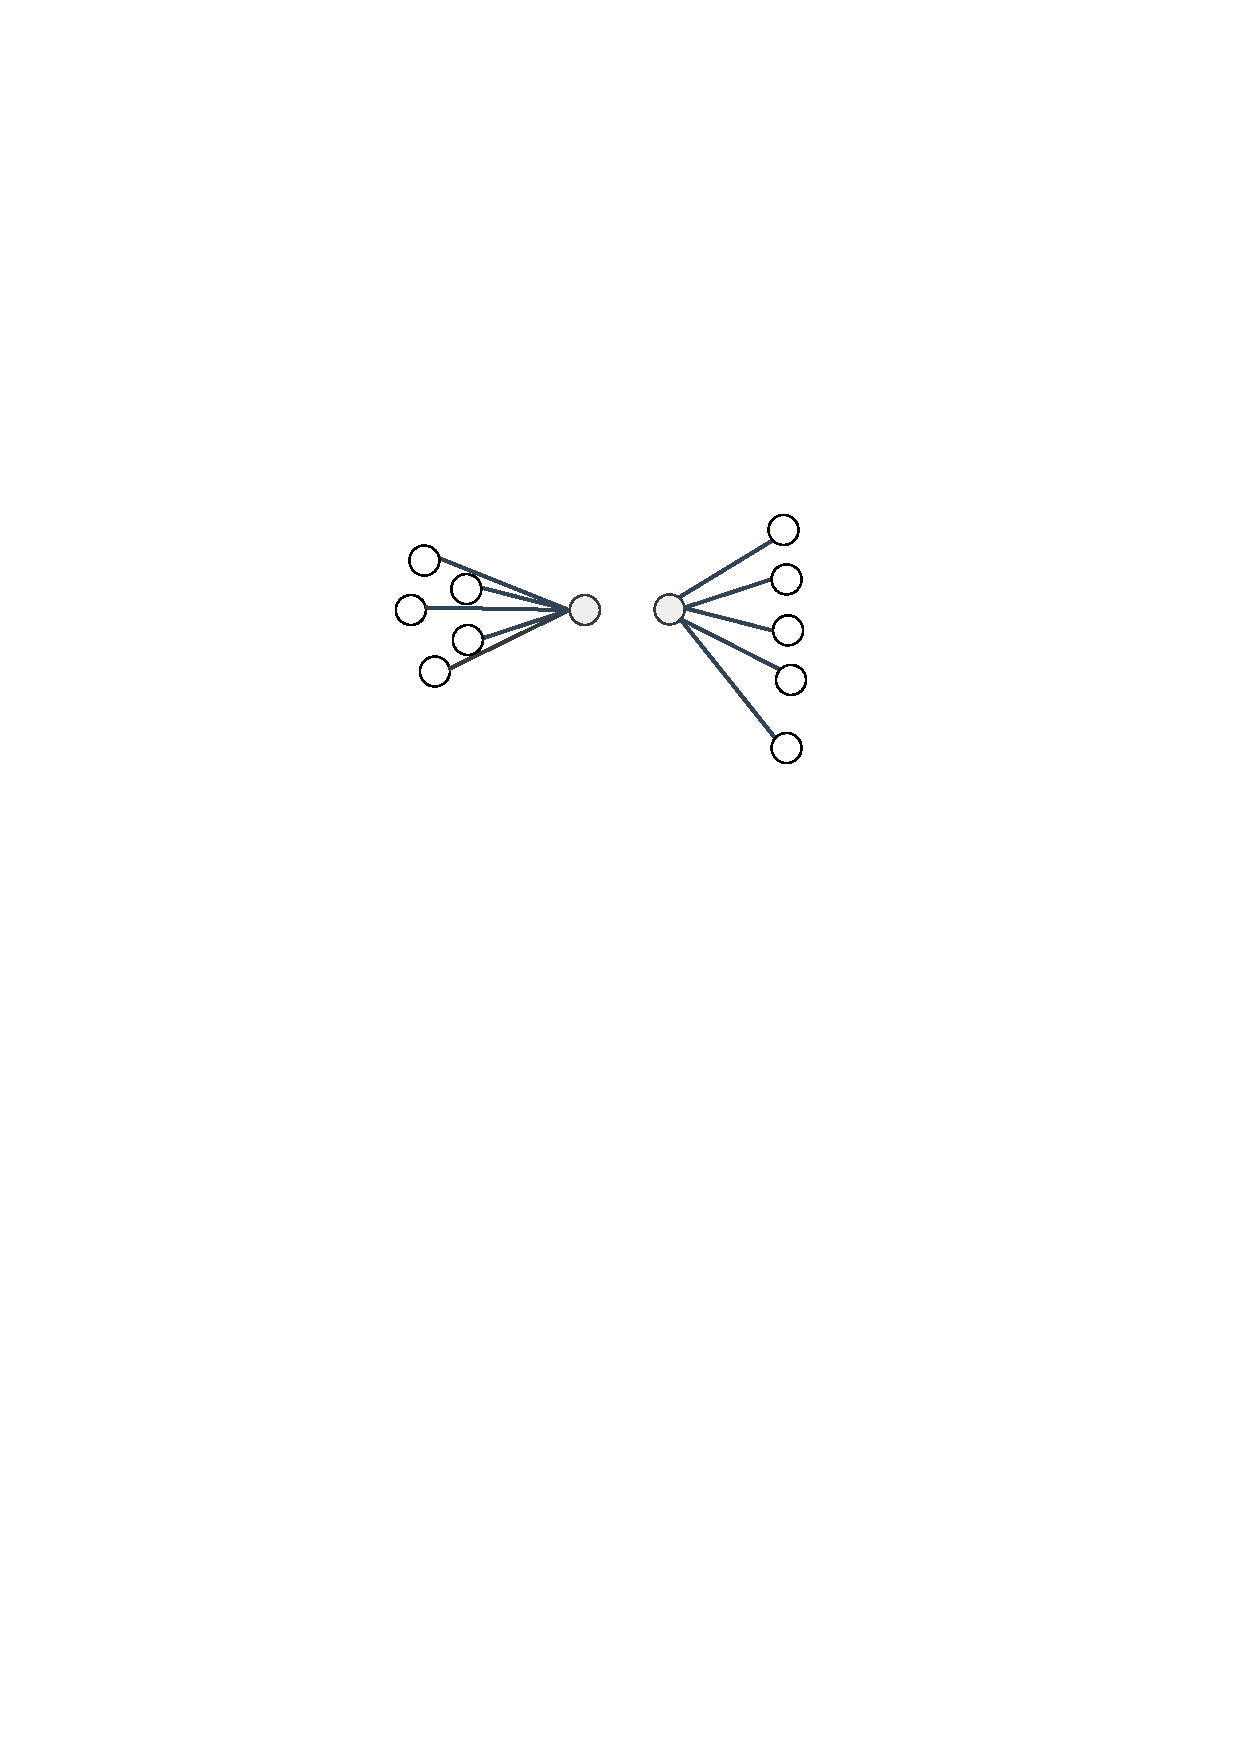
\includegraphics[scale=.6]{figures/followers/follower1}
% \label{fig:follower1}}
% \quad
% 	\subfloat[][\textbf{... but different number of followers' followers}]{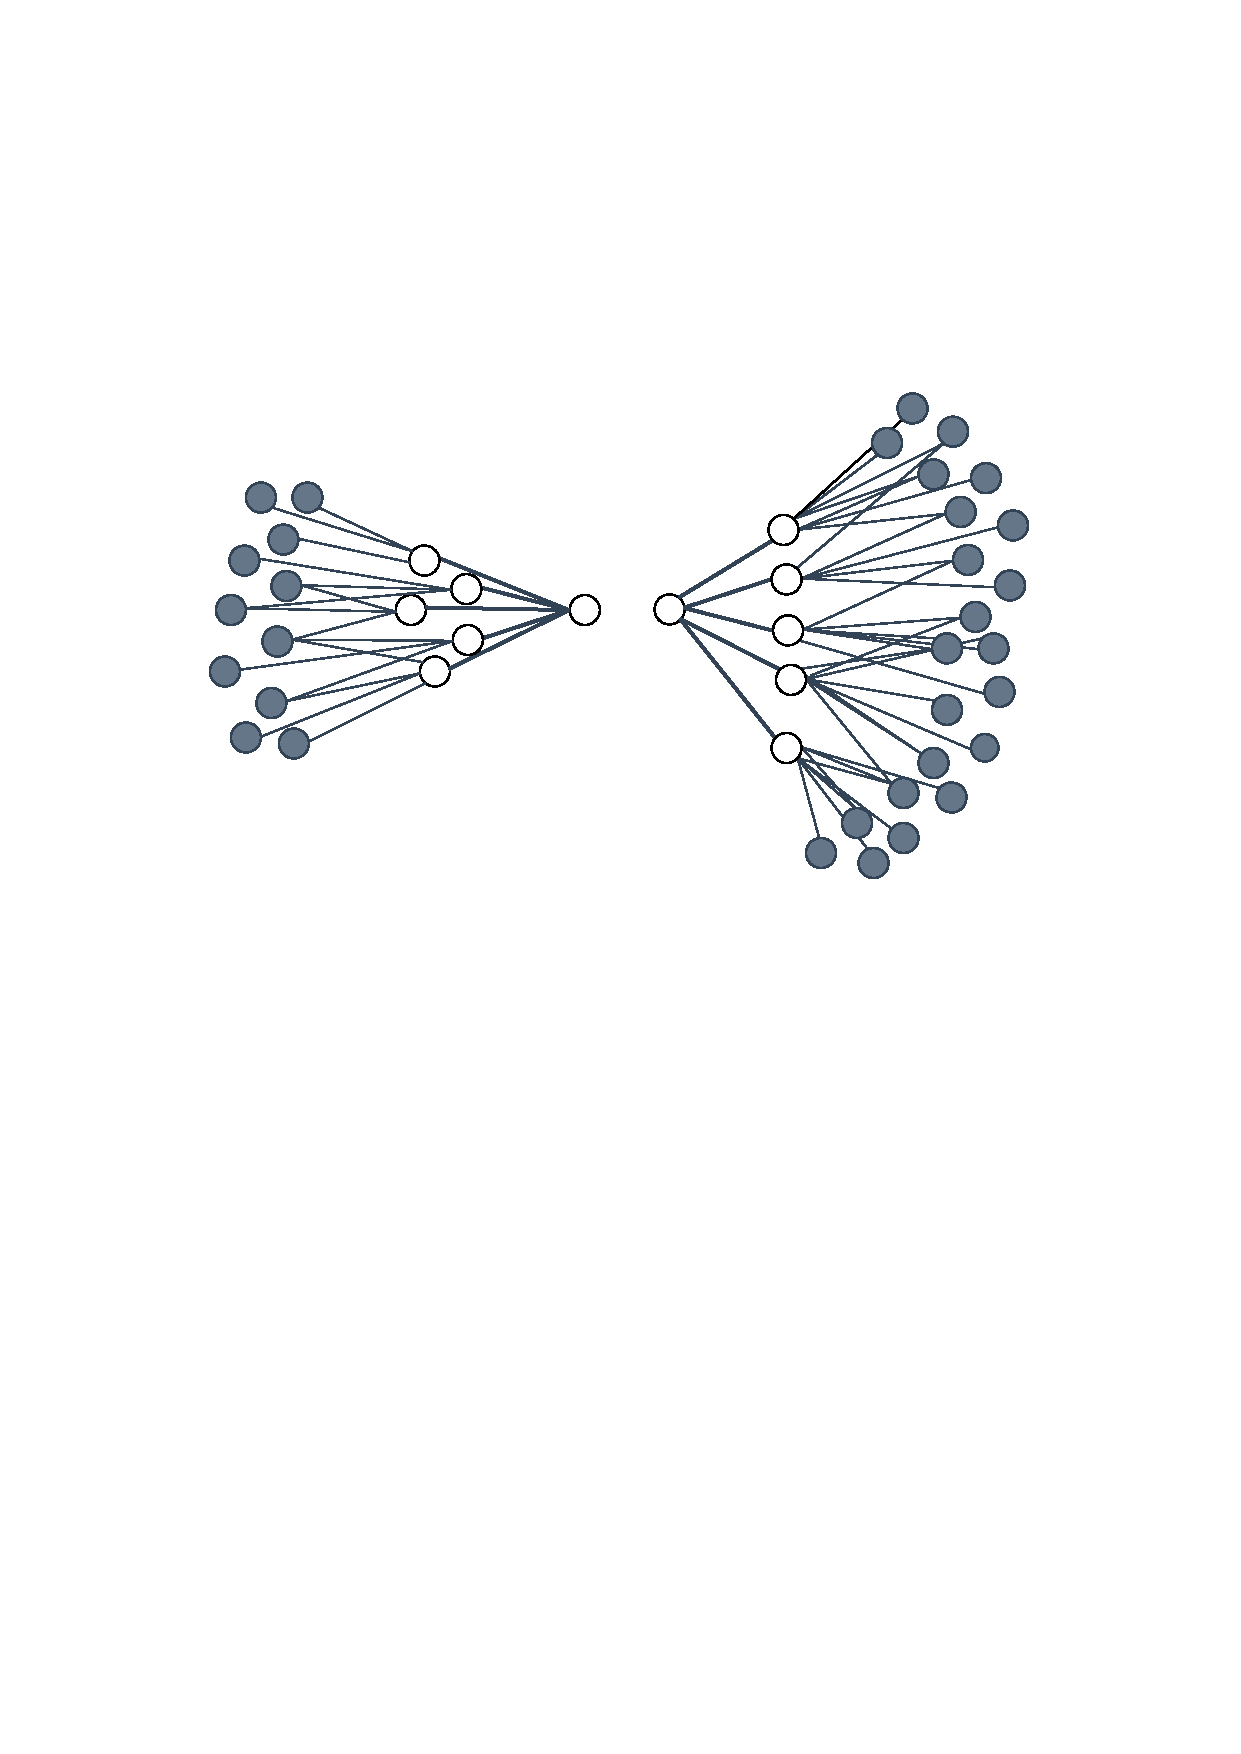
\includegraphics[scale=.6]{figures/followers/follower2}
% \label{fig:follower2}}
% \quad
% 	\subfloat[][\textbf{, leading to different number of tweets' impressions}]{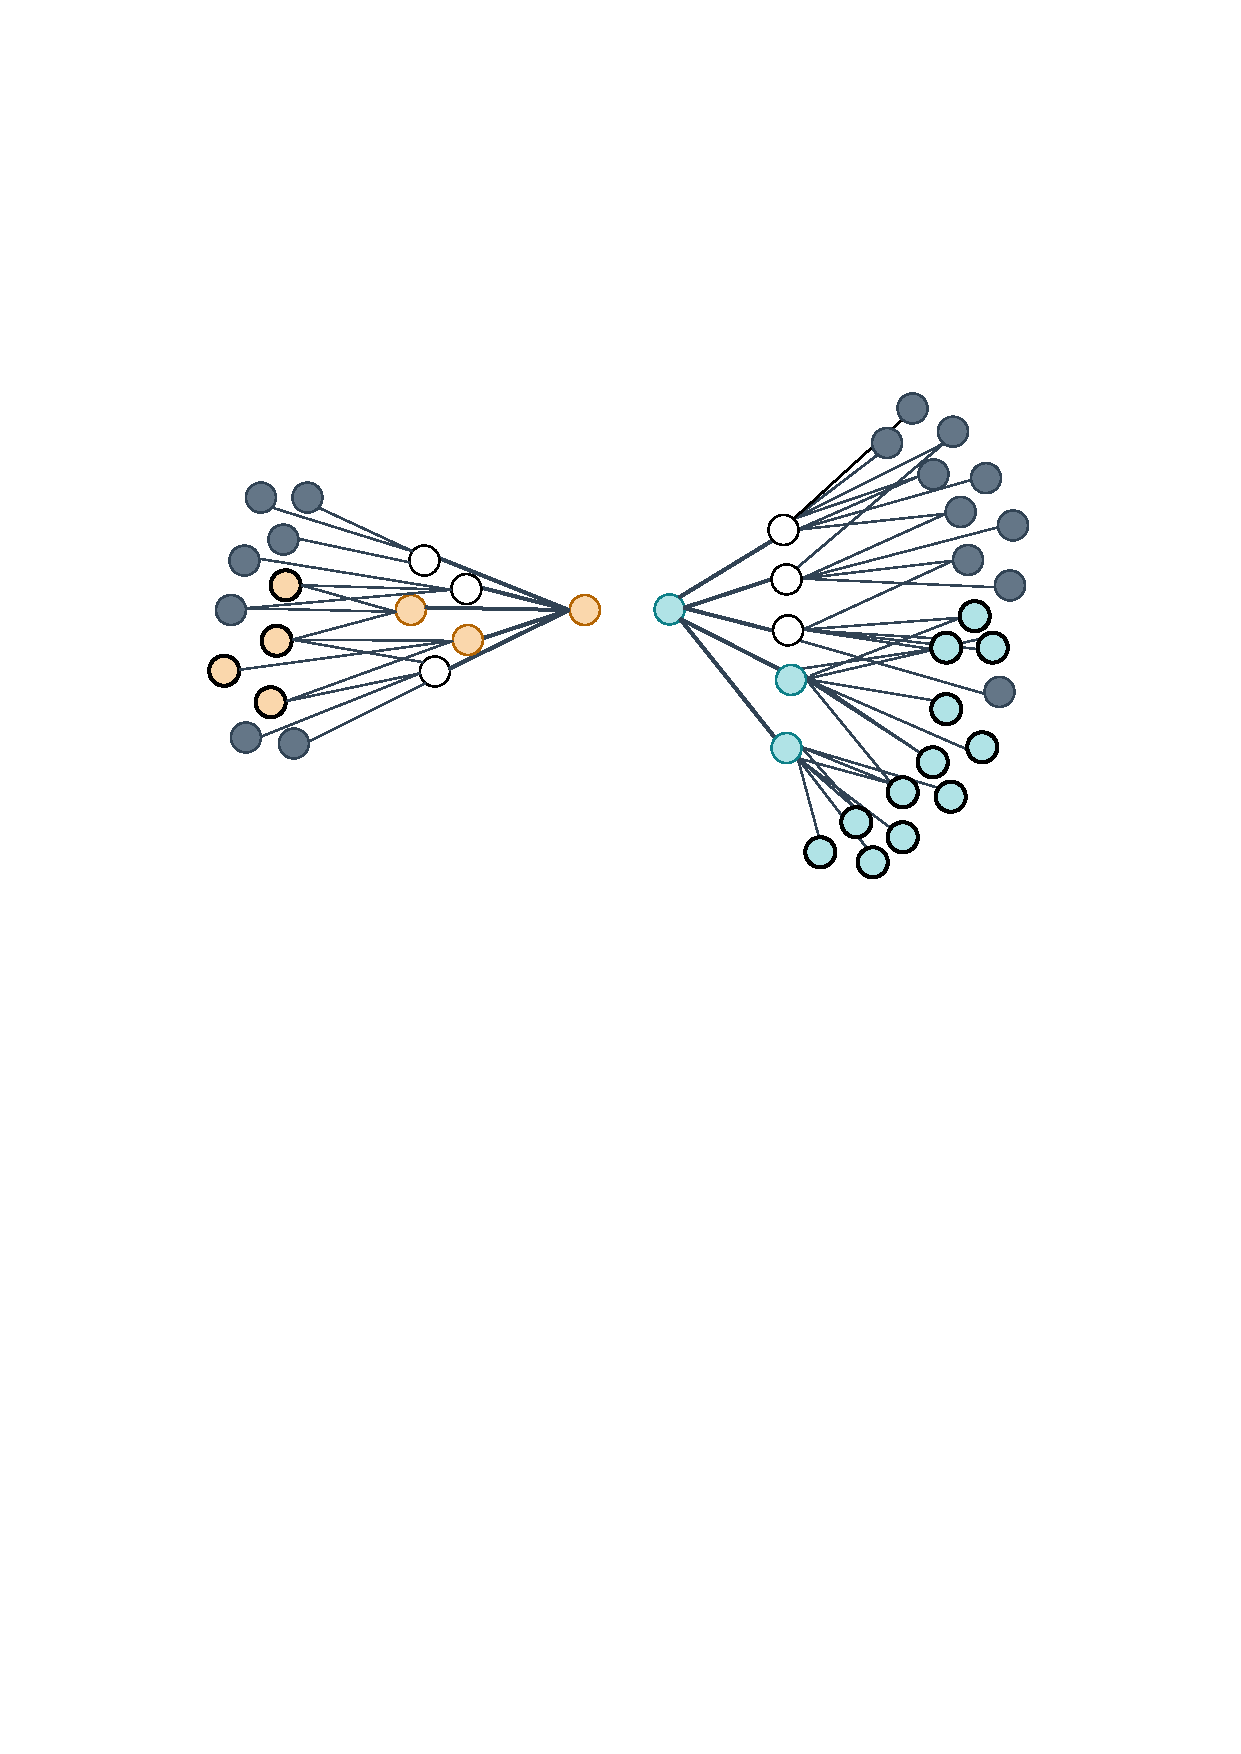
\includegraphics[scale=.6]{figures/followers/follower3}
% \label{fig:follower3}}
% \end{center}
% 	\begin{spacing}{0.5}
% 		{\footnotesize \textbf{Notes:} The Figure illustrates the IV strategy we develop in this article, in the spirit of an intention-to-treat approach. The thought experiment is described in details in the text.}
% 	\end{spacing}
% \vspace{.5cm}	
% 	\caption{IV strategy: Illustration}
% 	\label{fig:follower}
% \end{figure}
% %%%%%%%%%%%%%%%%%%%%%%%%%%%%%%%%%%%%%%%%%%%%%%%%%%%%%%%%%%%%%%%%%%%%%% 


However, while presumably more exogenous than the previous approach, the number of impressions generated by the seeds' followers may still suffer from the fact that a seed's centrality in the Twitter network may be related to it's ability to produce newsworthy content. To relax the exclusion restriction, the instrument we propose is the interaction between the seed's centrality in the network (as previously defined) and the news pressure at the time of the tweet (measured by the number of interactions generated by all the tweets published in the hour preceding the tweet), controlling for the direct effect of centrality and news pressure.\footnote{We thanks Katia Zhuravskaya for suggesting us this approach.} Our identification assumption is that, once we control for the direct effects of centrality and news pressure, the interaction between the seed's centrality and news pressure should only affect traditional news production through its effect on the tweet's visibility on Twitter.
% (if you control for the direct effect of the centrality, which could be correlated with the quality of the content, and for the news pressure, which could affect both the twitter users' and the media's attention at the same time.)


We show that, at the event-level, a $1,000$-increase in the number of tweets published before the first media article is associated with an increase by $2$ in the number of media articles published in the event; this increase is partly driven by an higher number of media outlets covering the event. Importantly, these results are robust to controlling for the endogeneity of the event popularity on Twitter, and to the use of a number of different empirical specifications.

We then turn to the media-level analysis and investigate the heterogeneity of our resultson the characteristics of the media outlets. For each of the media outlets in our sample, we collect information on their social media presence, as well as on their business model (e.g. whether they put part of their content behind a paywall and their reliance on advertising revenues). Besides, for a subset of the media, we also gather information on the size of their newsroom, which provides us a proxy on their investment in news quality. Ultimately, we also investigate whether there is heterogeneity depending on the offline format of the media. We show that the magnitude of the effect is stronger for the media whose social media presence is relatively higher.
%  depending on the topic of the event (e.g. sport, international affairs, economics, etc.), as well as 
% We find that \textbf{A COMPLETER} 

Finally, we discuss the mechanisms that may help rationalizing our findings. First, journalists monitor Twitter. E.g., the Muck Rack’s  ``State of Journalism 2019" report reveals that nearly $60\%$ of reporters turn to digital newspapers or magazines as their first source of news, and $22\%$ check Twitter first. This may help understanding why a number of stories emerge first on Twitter and the high reactivity of mainstream media, but not why the intensity of the media coverage (on the intensive margin) varies with the popularity of a story on Twitter. In the absence of perfect information about consumer preferences, publishers may use Twitter as a signal that allows them to draw inferences about what news consumers are interested in. Finally, social media and mainstream media compete for readers' attention. This may affect mainstream media incentives to invest in quality.


%%%%%%%%%%%%%%%%%%%%%%%%%%%%%%%%
\paragraph{Literature review}

This paper contributes to the growing literature on the impact of the introduction of new media technologies on political participation, government accountability and electoral outcomes (see among others \citet{Gentzkowetal2011,SnyderStromberg2010} on newspapers; \citet{Stromberg2004} on radio; \citet{Gentzkow2006,AngelucciCage2019,AngelucciCageSinkinson2020} on television, and \citet{BoxellGentzkowShapiro2018,Gavazzaetal2019} on the Internet). Only a few papers examine how social media affects voting \citep[for a review of the literature see][]{Zhuravskayaetal2020}, and they mainly concentrate on the role played by fake news \citep{AllcottGentzkow2017}. Until now, the focus of this literature has mostly been on news consumption, and little is known on the empirical impact social media have on news production by mainstream media. An exception is a work-in-progress article by \citet{HatteMadinierZhuravskaya2020}  who study the effect of Twitter on the US  TV coverage of the Israeli-Palestinian conflict. Compared to this work, our contribution is threefold. First, we focus on the overall activity on Twitter and collect a large representative sample of about 70\% of all Tweets (about $1.8$ billion Tweets) rather than the tweets associated with a small number of keywords. Second, we develop an instrument for measuring popularity shocks on Twitter based on the structure of the network that could be of use in different contexts rather than relying on an Internet outage instrument (which affects all electronic communications, access to online media, etc., and not only access to Twitter). Finally, we investigate whether there are heterogeneous effects depending on the media characteristics, in particular their business model and their reliance on advertising revenues.

An expanding theoretical literature studies the effects of social media on news. \Citet{deCorniereSarvary2019} develop a model where consumers allocate their attention between a newspaper and a social platform \citep[see also][for a theory of news coverage in environments of information abundance]{AlaouiGermano2020}. They document a negative impact on medias' incentives to invest in quality. This literature mainly concentrates on competition for attention between newspapers and social media, and documents a trade-off between the business-stealing and the readership-expansion effect of platforms \citep{JeonNasr2016}.\footnote{See \citet{Jeon2018} for a survey of articles on news aggregators.}  In this article, we highlight that not only mainstream and social media are competing for attention, but that social media can be used by mainstream media as a source of news as well as a signal to draw inferences on consumers' preferences. We investigate empirically how a story popularity on Twitter impacts the information produced by traditional media, and in particular the intensity of the coverage they devote to this story.

Our results also contribute to the growing literature in Economics and in Political science using social media data, and in particular the structure of the social networks -- most often Twitter -- as a source of information on the ideological positions of actors \citep{Barbera2015,cardon2019unfolding}, the importance of ideological segregation and the extent of political polarization \citep{HalberstamKnight2016,Giavazzietal2020}, or political language dissemination \citep{Longhietal2019}.\footnote{See also \citet{Barberaetal2019} who use Twitter data to analyze the extent to which politicians allocate attention to different issues before or after shifts in issue attention by the public.} \citet{Gorodnichenkoetal2018} study information diffusion on Twitter, and \citet{AllcottGentzkowYu2019_ReasearchPolitics} the spread of false content. While this literature mostly focuses on relatively small corpuses of tweets and on corpuses that are not representative of the overall activity on Twitter \citep[e.g.][make requests to collect tweets using Brexit-related keywords]{Gorodnichenkoetal2018}, in this paper, we build a representative corpus of tweets and impose no restriction on the data collection. Further, we contribute to this literature by considering not only the propagation of information on social media but also by studying whether and how information propagates from social media to mainstream media (and the other way around). While \citet{CageHerveViaud2020} only consider news propagation on mainstream media, we investigate here the extent to which the popularity of a story on social media affects the coverage devoted to this story by traditional media outlets.

The impact of ``popularity" on editorial decisions has been studied by \citet{SenYildirim2015} who use data from an Indian English daily newspaper to investigate whether editors expand online coverage of stories which receive more clicks initially.\footnote{See also \citet{ClaussenPeukertSen2019} who use data from a German newspaper to investigate whether automated personalized recommendation outperforms human curation in terms of user engagement.} Compared to this previous work, our contribution is threefold. First, we use the entire universe of French general information media online (around $200$ media outlets), rather than one single newspaper. Second, we identify not only the role played by popularity, but also investigate whether there is heterogeneity depending on the characteristics of the media outlets, as well as the topic of the story. Third, we consider both the extensive and the intensive  margin\footnote{The intensive margin here corresponds to whether a story is covered, while on the extensive margin we consider both the total number of articles (conditional on covering the story) and the characteristics of these articles.}, rather than focusing on the subset of stories that receive at least some coverage in the media. Finally, we also contribute to the empirical literature on media by using a split-sample approach; while this approach is increasingly used in economics with the pre-registration of Randomized Controlled Trials, we think we are the very first to use it with ``real-world data" on such a large scale.

Besides, we contribute to the broader literature on social media that documents its impact on racism \citep{MullerSchwarz2019}, political protests \citep{EnikolopovMakarinPetrova2020}, the fight against corruption \citep{Enikolopovetal2018}, or the size of campaign donations \citep{Petrovaetal2017}. Overall, social media is a technology that has both positive and negative effects \citep{Allcottetal2020}. This also holds true for its impact on traditional media: we contribute to this literature by documenting the complex effects social media has on news production, and consequently on news consumption.

Finally, our instrumentation strategy is related on the one hand to the literature that look at the quantity of newsworthy material at a given moment of time \citep[e.g.][]{EisenseeStromberg2007,DjourelovaDurante2019}, and on the other hand to the literature on network interactions \citep[see][for a recent survey]{BramoulleDjebbariFortin2020}. The main issue faced by researchers willing to identify the causal effects of peers is that the structure of the network itself may be endogenous. In this paper, we relax the concern of network endogeneity by considering the interaction between the network and news pressure at a given moment of time.


\medskip
The rest of the paper is organized as follows. In Section \ref{Sec:DataAlgorithms} below, we describe the Twitter data and the news content data we use in this paper, and review the algorithms we develop to study the propagation of information between social and mainstream media, and provide new descriptive evidence on news propagation. In Section \ref{Sec:EmpiricalSpecification}, we present our empirical specification, and in particular the new instrument we propose to identify the causal impact of a story popularity on the subsequent news coverage it receives. Section \ref{Sec:Results} presents the results and analyzes various dimensions of heterogeneity. In Section \ref{Sec:Mechanisms}, we discuss the mechanisms at play. Finally, Section \ref{Sec:Conclusion} concludes.


%%%%%%%%%%%%%%%%%%%%%%%%%%%%%%%%%%%%%%%%%%%%%%%%%%%%%%%%%%%%%%%%
%%%%%%%%%%%%%%%%%%%%%%%%%%%%%%%%%%%%%%%%%%%%%%%%%%%%%%%%%%%%%%%%
\section{Data, algorithms, and descriptive statistics\label{Sec:DataAlgorithms}}
%%%%%%%%%%%%%%%%%%%%%%%%%%%%%%%%%%%%%%%%%%%%%%%%%%%%%%%%%%%%%%%%
%%%%%%%%%%%%%%%%%%%%%%%%%%%%%%%%%%%%%%%%%%%%%%%%%%%%%%%%%%%%%%%%

The new dataset we built for this study is composed of two main data sources that we have collected and merged together: on the one hand, a representative sample of tweets, and on the other hand, the online content of the general information media outlets. In this section, we describe these two datasets in turn, and then present the algorithms we develop to identify events on social and on traditional media, and interact them.


%%%%%%%%%%%%%%%%%%%%%%%%%%%%%%%%%
\subsection{Data: Tweets\label{Sec:DataTweets}}
%%%%%%%%%%%%%%%%%%%%%%%%%%%%%%%%%

First, we collect a representative sample of all the tweets in French during an entire year: July 2018 - July 2019. Our dataset, which contains around $1.8$ billion tweets, encompasses around $70\%$ of all the tweets in French (including the retweets) during this time period.\footnote{See below for a discussion of the completeness of our dataset.} For each of these tweets, we collect information on their ``success" on Twitter (number of likes, of comments, etc.), as well as information on the characteristics of the user at the time of the tweet (e.g. its number of followers).

To construct this unique dataset, we have combined the Sample and the Filter Twitter Application Programming Interfaces (APIs), and selected keywords. Here, we quickly present our data collection strategy; more details are provided in \citet{Mazoyer2018,mazoyer2020french} and we summarize of data collection setup in the online Appendix Figure \ref{Figure:ExperimentalSetup}. 


%%%%%%%%%%%%%%%%%%%%%%%%%%%%%%%%%
\subsubsection{Data collection strategy\label{Sec:DataCollectionStrategy}}

There are different ways of collecting large volumes of tweets, although collecting the full volume of tweets emitted during a given period is not possible. Indeed, even if Twitter is known for providing a larger access to its data than other social media platforms, the Twitter streaming APIs are strictly limited in term of volume of returned tweets. The Sample API continuously provides $1\%$ of the tweets posted around the world at a given moment of time \citep[see e.g.][]{kergl_endogenesis_2014,morstatter_when_2014}. The Filter API continuously provides the same volume of tweets ($1\%$ of the global volume of tweets emitted at a given moment), but corresponding to the input parameters chosen by the user, including keywords, account identifiers, geographical area, as well as the language of the tweets.

To maximize the size of our dataset, we identify the keywords that maximize the number of returned French tweets as well as their representativity of the real Twitter activity. The selected terms had to be the most frequently written words on Twitter, and we had to use different terms (and terms that do not frequently co-occur in the same tweets) as parameters for each API connection. To do so, we extract the vocabulary from a set of tweets collected using the Sample API and obtain a subset of the words having the highest document-frequency. From this subset, we build a word co-occurrence matrix and, using spectral clustering, extract  clusters of words that are then used as parameters of our different connections to the Filter API. By doing so, we group terms that are  frequently used together (and separate terms that are rarely used together) and thus collect sets of tweets with the smallest possible intersection.


%%%%%%%%%%%%%%%%%%%%%%%%%%%%%%%%%
\paragraph{Filtering the tweets}

An important issue on Twitter is the use of bots, i.e. non-human actors and trolls publishing tweets on the social media  \citep[see e.g.][]{Gorodnichenkoetal2018}. In recent years, Twitter has been actively cracking down on bots. In our analysis, we further identify and purge the bots.\footnote{However we do not remove all automatically publishing accounts: many media accounts, for example, post some content automatically, and are not considered as bots. Moreover, some types of automatic behaviors on Twitter, such as automatic retweets, may contribute to the popularity of stories and therefore should be kept in our dataset.}

To do so, we proceed as follows. First, we filter the tweets using the ``source" metadata provided by Twitter. Tweets emanating from a ``source" such as ``Twitter for iPhone" can be considered as valid; however, we excluded sources such as ``ManageTweetBot" and ``Random Taxi bot". We also excluded apps automatically posting tweets based on the behaviour of users: for example, many Twitter users (that are human beings and usually publish tweets they have written themselves) post automatic tweets such as ``I like a video on Youtube: [url]". Second, we filter the users depending on their activity on the network: we only keep users with less than $1,000$ tweets a day\footnote{As a matter of comparison, the Twitter account of \textit{Le Monde} publishes on average $88$ tweets per day, and the one of \textit{Le Figaro} 216.}, and the users who have at least 1 follower. Finally, we only keep the users who have at least 3 tweets in French between July and September 2018.


%%%%%%%%%%%%%%%%%%%%%%%%%%%%%%%%%
\paragraph{Completeness of the dataset}

Ultimately, we obtain $1.8$ billion tweets in French between July 2018 and July 2019. While the objective of our data collection method was to maximize the number of tweets we collect -- and given we do not know the actual number of tweets emitted in French during the same time period --, we need to use other corpora to get a sense of the completeness of our dataset. We rely on three different metrics to estimate the share of the tweets that we collect (respectively miss).

The DLWeb, i.e. the French Internet legal deposit department at the INA (\textit{Institut National de l'Audiovisuel} -- National Audiovisual Institute, a repository of all French radio and television audiovisual archives) is in charge of archiving French websites related to audiovisual media, and also collects tweets concerning audiovisual media by using a manually curated list of hashtags and Twitter accounts. We compare our dataset of tweets with the tweets they collected for 25 hashtags in December 2018. We find that on average, we collected $74\%$ of the tweets from the DLWeb, and $78\%$ if we exclude retweets\footnote{Original tweets are better captured than retweets by our collection method, because each retweet allows us to archive the original tweet to which it refers. Therefore, we only need to capture one of the retweets of a tweet to get the original tweet. Retweets, on the other hand, are not retweeted, so we lose any chance of catching them if they were not obtained at the time they were sent.} (see online Appendix Figure \ref{Figure:HistogramHashtagsDLWeb} for more details).

Second, we compare our dataset with the corpus of tweets built by \citet{cardon2019unfolding}, that consists of tweets containing URLs from a curated list of 420 French media outlets. \citet{cardon2019unfolding} provide us with all tweets they collect in December 2018, i.e. $8.7$ million tweets, out of which $7.3$ million tweets in French. Our dataset contains $70\%$ of these tweets in French, $74\%$ if we exclude retweets (see online Appendix Figure \ref{Figure:HistogramUrlsMedialab}).

Finally, our third evaluation method is based on the total number of tweets sent by a user since the account creation, a metadata that is provided by Twitter for every new tweet. With this metric, we can get an estimate of the total number of tweets emitted by a given user between two of her tweets. We can then compare this value with the number of tweets we actually collect for that user. In practice, we selected the tweets of all users located in France.\footnote{See the online Appendix Section \ref{Sec:OA_Tweet} for more details. We focus on the users located in France given they have a higher probability to only publish tweets in French, and we only capture here by construction the tweets in French.} We find that our dataset contains $61\%$ of the real number of emitted tweets for these users. This evaluation is a low estimate of the percentage of collected tweets, since some users located in France may write tweets in other languages than French. 

All three comparison methods have their flaws, however they produce close results. We can therefore conclude that we collect between $60\%$ and $75\%$ of all tweets in French during our time period. To the extent of our knowledge, there is no equivalent in the literature of such a dataset of tweets, in terms of size and representativity of the Twitter activity. We hope that both our methodology and data could be of use in the future to other researchers.


%%%%%%%%%%%%%%%%%%%%%%%%%%%%%%%%%
\subsubsection{Descriptive statistics}

%Table \ref{Tab:sum_stat_tweets_201809_201902} provides summary statistics on the tweets we collected. For each of the tweets, we have information of their length ($101$ characters on average or $6.1$ words), and know whether the tweet is a retweet of an existing tweet or an original tweet. $63\%$ of the tweets in our dataset are retweets; some of these retweets are ``quotes", i.e. comment on the retweeted tweet.\footnote{Quote Tweets share another tweet with an additional comment, unlike Retweets that repost the original tweet without any modification.} Among the original tweets, some are in reply to other tweets ($18\%$ of the tweets in our sample). Finally, $12\%$ of the tweets contains an URL, most often a link to a news media article or to a video.
%
%We also gather information on the popularity of each of the tweets in our sample. On average, the tweets are only retweeted $0.8$ times, liked $1.5$ times, and receive $0.1$ replies (these numbers are only computed on the original tweets, given retweets, likes and quotes are not attributed to the Retweets but to the original tweets).
%
%
%%%%%%%%%%%%%%%%%%%%%%%%%%%%%%%%%%%%%%%%%%%%%%%%%%%%%%%%%%%%%%%%%%%%%%%
%\begin{sidewaystable}
%\caption{Summary statistics: Tweets (full sample) \textbf{COMPLETER AVEC LA VERSION A JOUR -- ET RAJOUTER EGALEMENT STAT DES SUR FULL SAMPLE OF USERS}}
%\begin{center}
%	{
\def\sym#1{\ifmmode^{#1}\else\(^{#1}\)\fi}
\begin{tabular}{l*{1}{ccccccc}}
\hline\hline
                    &\multicolumn{7}{c}{}                                                                      \\
                    &        Mean&      St.Dev&         P25&      Median&         P75&         Max&         Obs\\
\hline
\textbf{Characteristics of the tweet}&            &            &            &            &            &            &            \\
Length of the tweet (nb of characters)&         101&          54&          59&          97&         140&       1,415&1,030,423,899\\
Number of words     &         6.1&         4.1&         3.0&         6.0&         8.0&       269.0&1,030,423,899\\
=1 if tweet contains an URL&        0.12&        0.33&        0.00&        0.00&        0.00&        1.00&1,030,423,899\\
=1 if the tweet is a retweet&        0.63&        0.48&        0.00&        1.00&        1.00&        1.00&1,030,423,899\\
=1 if the tweet is a reply&        0.18&        0.39&        0.00&        0.00&        0.00&        1.00&1,030,423,899\\
=1 if the tweet is a quote&        0.20&        0.40&        0.00&        0.00&        0.00&        1.00&1,030,423,899\\
\textbf{Popularity of the tweet}&            &            &            &            &            &            &            \\
Number of retweets  &         0.8&        65.8&         0.0&         0.0&         0.0&   365,931.0&1,030,423,897\\
Number of replies   &         0.1&         5.0&         0.0&         0.0&         0.0&    49,218.0&1,030,423,897\\
Number of likes     &         1.5&       115.8&         0.0&         0.0&         0.0&   980,681.0&1,030,423,899\\
\textbf{Characteristics of the user}&            &            &            &            &            &            &            \\
Total nb of Tweets  &      35,798&     300,554&       2,312&       9,902&      32,403&  20,389,037&1,030,423,899\\
Nb of followers     &       3,225&      73,841&          96&         279&         742& 106,815,712&1,030,423,899\\
Nb of users the account is following&         669&       3,946&         124&         258&         559&   1,829,616&1,030,423,899\\
=1 if user is a media&       0.001&       0.036&       0.000&       0.000&       0.000&       1.000&1,030,423,899\\
=1 if user is a journalist&       0.002&       0.043&       0.000&       0.000&       0.000&       1.000&1,030,423,899\\
\hline\hline
\end{tabular}
}

%\end{center}
%\begin{spacing}{0.5}
%	{\fns \textbf{Notes:} The table gives summary statistics. Time period is July 2018 - July 2019. Variables are values for all the tweets included in our dataset. Variables are described in more details in the text.} 
%\end{spacing}
%\label{Tab:sum_stat_tweets_201809_201902}
%\end{sidewaystable} 
%%%%%%%%%%%%%%%%%%%%%%%%%%%%%%%%%%%%%%%%%%%%%%%%%%%%%%%%%%%%%%%%%%%%%%%
%

%%%%%%%%%%%%%%%%%%%%%%%%%%%%%%%%%
\paragraph{Split-sample approach}

As highlighted in the introduction, to address concerns about specification search and publication bias \citep{Leamer1978,Leamer1983,Glaeser2006_incentives}, we implement a split-sample approach in this paper \citep{FafchampsLabonne2016,FafchampsLabonne2017,AndersonMagruder2017}. We split the data into two non-overlapping datasets: July 2018 - September 2018 and October 2018 - July 2019. We used the three-month dataset covering July 2018 - September 2018 to narrow down the list of hypotheses we wished to test and prepared this draft of the paper.

The final version of the paper will only use data from October 2018 to July 2019. The idea here is to avoid multiple hypothesis testing that has been shown to be an issue in experimental economics \citep{ListShaikhXu2019}, and that could also be of concern here. Hence, for the remainder of the article, we will only rely on the first three months of our dataset. This sample includes $417,153,648$ tweets; Table \ref{Tab:sum_stat_tweets_split_sample} presents summary statistics for these tweets. 


%%%%%%%%%%%%%%%%%%%%%%%%%%%%%%%%%
\paragraph{Summary statistics}

For each of the tweets, we have information of their length ($102$ characters on average or $6.2$ words), and know whether the tweet is a retweet of an existing tweet or an original tweet. $63\%$ of the tweets in our dataset are retweets; some of these retweets are ``quotes", i.e. comment on the retweeted tweet.\footnote{Quote Tweets are much like Retweets except that they include a new Tweet message.} Among the original tweets, some are in reply to other tweets ($17\%$ of the tweets in our sample). Finally, $13\%$ of the tweets contains an URL, most often a link to a news media article or to a video.

We also gather information on the popularity of each of the tweets in our sample. On average, the tweets are retweeted $2.3$ times, liked $3.7$ times, and receive $0.2$ replies (these numbers are only computed on the original tweets, given retweets, likes and quotes are not attributed to the Retweets but to the original tweets).\footnote{Online Appendix Table \ref{Tab:sum_stat_tweets_split_sample_bflitre} shows statistics on the sample of tweets we collect before applying the filters to exclude the bots as described above.} 


%%%%%%%%%%%%%%%%%%%%%%%%%%%%%%%%%%%%%%%%%%%%%%%%%%%%%%%%%%%%%%%%%%%%%%
\begin{sidewaystable}
\caption{Summary statistics: Tweets (split-sample, July 2018-September 2018)}
\begin{center}
	{
\def\sym#1{\ifmmode^{#1}\else\(^{#1}\)\fi}
\begin{tabular}{l*{1}{ccccccc}}
\hline\hline
                    &\multicolumn{7}{c}{}                                                                      \\
                    &        Mean&      St.Dev&         P25&      Median&         P75&         Max&         Obs\\
\hline
\textbf{Characteristics of the tweet}&            &            &            &            &            &            &            \\
Length of the tweet (nb of characters)&         102&          52&          61&          98&         140&       1,121& 417,153,648\\
Number of words     &         6.2&         4.0&         3.0&         6.0&         9.0&         269& 417,153,648\\
=1 if tweet contains an URL&        0.13&        0.33&        0.00&        0.00&        0.00&           1& 417,153,648\\
=1 if the tweet is a retweet&        0.63&        0.48&        0.00&        1.00&        1.00&           1& 417,153,648\\
=1 if the tweet is a reply&        0.17&        0.38&        0.00&        0.00&        0.00&           1& 417,153,648\\
=1 if the tweet is a quote&        0.19&        0.39&        0.00&        0.00&        0.00&           1& 417,153,648\\
\textbf{Popularity of the tweet}&            &            &            &            &            &            &            \\
Number of retweets  &         2.3&       111.5&       0.000&       0.000&       0.000&     117,389& 154,273,618\\
Number of replies   &         0.2&         6.6&       0.000&       0.000&       0.000&      47,892& 154,273,618\\
Number of likes     &         3.7&       172.2&       0.000&       0.000&       0.000&     449,881& 154,273,619\\
\hline\hline
\end{tabular}
}

\end{center}
\begin{spacing}{0.5}
	{\fns \textbf{Notes:} The table gives summary statistics. Time period is July 2018 - September 2018. Variables are values for all the tweets included in our dataset. Variables for the ``popularity of the tweet" are only for the original tweets, given the retweets/replies/likes are always attributed to the original tweets (hence the lower number of observations). The maximum number of characters (or length of the tweet) is above the $280$ Twitter characters limit. This is due to the fact that URLs and mentions (e.g. $@BeatriceMazoyer$) contained in the tweets are not included by Twitter in the number of characters limit. We remove the stop-worrds before computing the ``number of words" statistics. The list of stop-words is provided in the online Appendix Section \ref{Sec:OA_Tweet}. Variables are described in more details in the text.} 
\end{spacing}
\label{Tab:sum_stat_tweets_split_sample}
\end{sidewaystable} 
%%%%%%%%%%%%%%%%%%%%%%%%%%%%%%%%%%%%%%%%%%%%%%%%%%%%%%%%%%%%%%%%%%%%%%

Further, we compute summary statistics on the Twitter users in our sample. Our dataset includes $4,222,734$ unique users between July 2018 and September 2018. Table \ref{Tab:table_summary_users_all_first} provides these statistics the first time a user is observed in our data.\footnote{Alternatively, we compute the users' characteristics the last time we observe them. The results are presented in the online Appendix Table \ref{Tab:table_summary_users_all_last}.} On average, the users have tweeted $14,100$ times, liked $7,463$ tweets, and follow $642$ other Twitter accounts. The average year of the account creation is 2014 (Twitter was created in 2006). (See online Appendix Figure \ref{fig:fig_nb_new_users_daily} for the distribution of the users depending on the date at which they have created their Twitter account.) On average, users have $2,166$ followers; however, we observe a lot of variation: the vast majority of the users only have a few followers, but some of them act as central nodes in the network: the top $1\%$ of the users in terms of followers  account for more than $70\%$ of the total number of followers (see online Appendix Figure \ref{fig:users} for the distribution of the number of followers).

$0.5\%$ of the users in our sample have a verified account\footnote{According to Twitter, an account may be verified if it is determined to be an account of public interest. Typically this includes accounts maintained by users in music, acting, fashion, government, politics, religion, journalism, media, sports, business, and other key interest areas.}, $0.12\%$ are the accounts of journalists, and $0.011\%$ are media outlets' accounts. We have manually identified the Twitter accounts of media outlets. For the Twitter accounts of journalists, we proceed to a semi-manual detection with the following method: first use the Twitter API to collect the name and description of all accounts that are followed by at least one Twitter media account. Second, we only keep the accounts having some keywords related to the profession of journalist in their description, such as ``journalist", ``columnist", ``news", etc. Third, we manually select journalists from the remaining accounts by reading their names and description.



%%%%%%%%%%%%%%%%%%%%%%%%%%%%%%%%%%%%%%%%%%%%%%%%%%%%%%%%%%%%%%%%%%%%%%
\begin{table}
\caption{Summary statistics: Twitter users}
\begin{center}
	{
\def\sym#1{\ifmmode^{#1}\else\(^{#1}\)\fi}
\begin{tabular}{l*{1}{cccccc}}
\hline\hline
                    &\multicolumn{6}{c}{}                                                         \\
                    &        Mean&      St.Dev&         P25&      Median&         P75&         Max\\
\hline
\textbf{User activity}&            &            &            &            &            &            \\
Total number of tweets&      14,100&      39,127&         192&       1,754&      11,228&   6,020,029\\
Nb of tweets user has liked&       7,463&      21,419&          95&         914&       5,414&   2,736,965\\
Nb of users the account is following&         642&       4,489&          76&         193&         482&   1,681,133\\
\textbf{User identity}&            &            &            &            &            &            \\
Date of creation of the account&        2014&           3&        2012&        2015&        2017&        2018\\
=1 if verified account&       0.005&       0.073&           0&           0&           0&           1\\
=1 if user is a journalist&       0.001&       0.034&           0&           0&           0&           1\\
=1 if user is a media&      0.0001&       0.010&           0&           0&           0&           1\\
\textbf{User popularity}&            &            &            &            &            &            \\
Nb of followers     &       2,166&      86,811&          24&         129&         477&  58,484,193\\
Nb of public lists  &          19&         578&           0&           1&           6&   1,028,761\\
\hline
Observations        &   4,222,734&            &            &            &            &            \\
\hline\hline
\end{tabular}
}

\end{center}
\begin{spacing}{0.5}
	{\fns \textbf{Notes:} The table gives summary statistics. Time period is July 2018 - September 2018. Variables are values for all the Twitter users included in our dataset the first time we observe them. Variables are described in more details in the text.} 
\end{spacing}
\label{Tab:table_summary_users_all_first}
\end{table} 
%%%%%%%%%%%%%%%%%%%%%%%%%%%%%%%%%%%%%%%%%%%%%%%%%%%%%%%%%%%%%%%%%%%%%%



%%%%%%%%%%%%%%%%%%%%%%%%%%%%%%%%%
\subsection{Data: News articles\label{Sec:DataNews}}
%%%%%%%%%%%%%%%%%%%%%%%%%%%%%%%%%

We combine the Twitter data with the online content of traditional media outlets (alternatively called mainstream media) over the same time period, including newspapers, radio channels, TV stations, online-only news media, and the content produced by the news agency ``Agence France Presse" (AFP). The goal here is to gather all the content produced online by the ``universe" of French news media, independently of their offline format. The data is collected as part of the OTMedia research project, a unique data collection program conducted by the French National Audiovisual Institute \citep{CageHerveViaud2020}. Further, we also gather the content produced online by $10$ French-speaking (non French) media outlets such as the daily newspaper \textit{Le Temps Suisse} from Switzerland. This subset of French-speaking media was selected based on the fact that the tweets included in our sample include at least one URL linked to an article published online by these media.


%%%%%%%%%%%%%%%%%%%%%%%%%%%%%%%%%
\paragraph{Newsrooms' characteristics}

Our dataset includes $205$ unique media outlets (see online Appendix Section \ref{Sec:OA_Content} for the list of these media depending on their offline format), that published online $929,764$ news articles between July 2018 and September 2018. Table \ref{Tab:sumstats_media} shows summary statistics for the mainstream media included in our dataset. On average, between July 2018 and September 2018, the mainstream media in our data published $4,152$ news articles (i.e. around $48$ articles per day), out of which $1,406$ are classified in events (see below for the event definition). $63.4\%$ of the articles come from the websites of the newspapers,  $13,1\%$ from pure online media, $11.1\%$ from the news agency, $8.8\%$ from the websites of the radio stations and the remainder from TV channels' websites (see online Appendix Figure \ref{fig:share_documents_used_media_category}.)


%%%%%%%%%%%%%%%%%%%%%%%%%%%%%%%%%%%%%%%%%%%%%%%%%%%%%%%%%%%%%%%%%%%%%%
\begin{table}
\caption{Summary statistics: Media outlets}
\begin{center}
	{
\def\sym#1{\ifmmode^{#1}\else\(^{#1}\)\fi}
\begin{tabular}{l*{1}{cccccc}}
\hline\hline
                    &\multicolumn{6}{c}{}                                                         \\
                    &        Mean&      St.Dev&         P25&      Median&         P75&         Max\\
\hline
\textbf{Content}    &            &            &            &            &            &            \\
Total content (thsd ch)&      10,021&      25,055&         414&       1,965&       8,045&     222,546\\
Total number of articles&       4,152&      10,035&         185&         837&       3,366&      85,676\\
Articles classified in events&       1,406&       4,524&          11&         114&         864&      55,932\\
Number of breaking news&        31.8&       135.0&         0.0&         0.0&        13.0&       1,656\\
\textbf{Online audience} (daily)&            &            &            &            &            &            \\
Number of unique visitors&     210,883&     301,686&      28,843&      90,153&     227,008&   1,282,498\\
Number of visits    &     586,269&     852,715&      72,165&     210,473&     714,832&   3,283,491\\
Number of pages views&   1,510,024&   2,544,652&     160,117&     536,866&   1,643,809&  15,329,183\\
\textbf{Social media presence}&            &            &            &            &            &            \\
\% articles on Twitter&          17&          17&           4&          10&          24&          70\\
Number of Twitter accounts&         3.1&         5.7&         1.0&         1.0&         2.0&          43\\
Date of Twitter account creation&        2009&         1.3&        2009&        2009&        2010&        2016\\
Number of tweets    &       2,874&       4,587&         455&       1,101&       3,043&      19,730\\
Nb journalists with Twitter account&         211&         354&          38&          81&         220&       3,086\\
\textbf{Other media characteristics}&            &            &            &            &            &            \\
Year of media creation&        1975&          39&        1945&        1986&        2008&        2018\\
Year of website creation&        2004&           7&        1998&        2004&        2010&        2018\\
Year of the paywall introduction&        2014&           5&        2013&        2015&        2018&        2020\\
Number of journalists&         147&         183&          32&          90&         208&        1121\\
\hline
Observations        &         205&            &            &            &            &            \\
\hline\hline
\end{tabular}
}

\end{center}
\begin{spacing}{0.5}
	{\fns \textbf{Notes:} The table gives summary statistics. Time period is July 2018 - September 2018. Variables are values for media outlets. The observations are at the media outlet/day level for the online audience statistics, and at the media outlet level for the content data and other media characteristics.} 
\end{spacing}
\label{Tab:sumstats_media}
\end{table} 
%%%%%%%%%%%%%%%%%%%%%%%%%%%%%%%%%%%%%%%%%%%%%%%%%%%%%%%%%%%%%%%%%%%%%%


For all the media outlets in our sample, we also collect information on their social media presence. First, we identify their Twitter account(s) (some media only have one Twitter accounts, while others have many; e.g. \textit{Le Monde}: $@lemondefr$, $@lemondelive$, $@lemonde\_pol$, etc.) and collect information on their popularity (number of followers and of public lists, the first time we observe them in our sample), as well as  the number of tweets tweeted by these accounts during our period of interest (July-September 2018). On average, the media outlets in our sample have $3.1$ different Twitter accounts. We compute the date of creation of each of these accounts, and report the oldest one in the table. To proxy for the media outlets' social media presence,  we also compute the share of the articles the media publishes online that are also on Twitter (see online Appendix Figure \ref{fig:fig_mean_Tweeted} for this statistic by media outlet). Besides, for each of the media in our sample, we compute the number of journalists with a Twitter account, as well as the characteristics of these accounts.
%  \textbf{[TO BE COMPLETE -- check with Beatrice for the data]} 

Second, to better understand the mechanisms that may be at play, we collect a number of additional information on the media: (i) their year of creation, (ii) the year of creation of their website (2004 on average), as well a (iii) information on their business model. In particular, for each of the media outlet, we investigate whether they use a paywall, conditional of having a paywall, the characteristics of this paywall (e.g. soft vs. hard), and the date of introduction of the paywall. This information is summarized on Figure \ref{fig:paywall_final}: while $48.1\%$ of the media outlets do not have a paywall, $43.1\%$ lock at least some of their articles behind a paywall (soft paywall). Metered paywall and hard paywall are much less frequent. The media outlets that use a paywall have introduced it on average in 2014. Overall, the large majority of the media outlets in our sample relies at least partly on advertising revenues; however, some of them do not (e.g. the pure online media Mediapart).
% A RAJOUTER (quand les donnees seront pretes -- Michel G.): estimated share of total revenues that comes from advertising


%%%%%%%%%%%%%%%%%%%%%%%%%%%%%%%%%%%%%%%%%%%%%%%%%%%%%%%%%%%%%%%%%%%%%%
\begin{figure}
\begin{center}
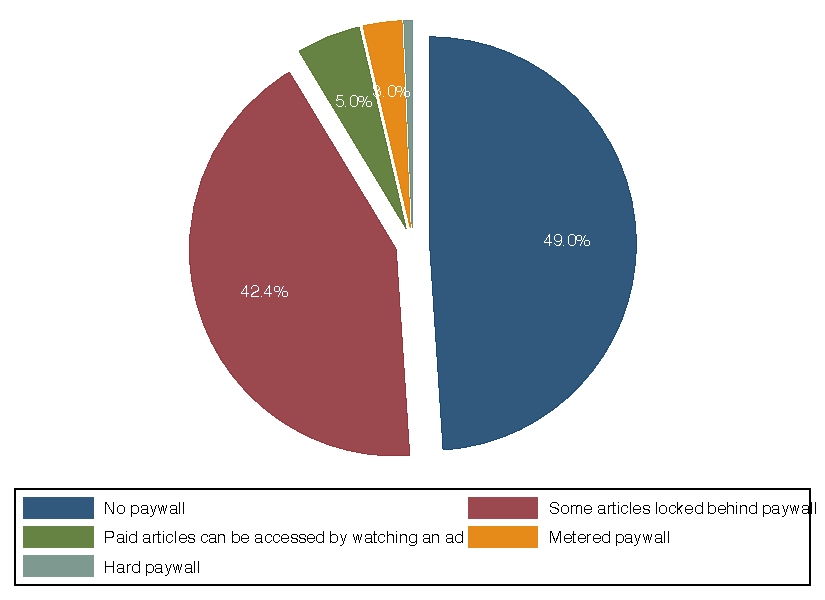
\includegraphics[scale=1]{figures/paywall_final}
\end{center}
	\begin{spacing}{0.5}
		{\footnotesize \textbf{Notes:} The Figure reports the share of the media outlets in our sample depending on their online business model. 48.1\% of the media in our sample do not have paywall (``no paywall"), and $5.1\%$ condition the reading of the paid articles on the fact of watching an ad (``paid articles can be accessed by watching an ad"). Among the outlets that do have a paywall, we distinguish between three models: hard paywall, metered paywall, and soft paywall (``some articles locked behind paywall).}
	\end{spacing}
\vspace{.5cm}	
	\caption{News editors business model}
	\label{fig:paywall_final}
\end{figure}
%%%%%%%%%%%%%%%%%%%%%%%%%%%%%%%%%%%%%%%%%%%%%%%%%%%%%%%%%%%%%%%%%%%%%% 


Third, given media outlets may react differently to social media depending on their initial investment in quality \citep[see e.g.][]{deCorniereSarvary2019}, we also compute information on the size of the newsroom, and on the average payroll \citep{Cage2015_journalists}. This information is available for $68$ media outlets in our sample. Finally, for the $72$ media outlets for which this information is available, we collect daily audience information from the ACPM, the French press organization whose aim is to certify circulation and audience data. The average number of daily visitors is $588,722$, and the average number of page views $1,524,534$.


%%%%%%%%%%%%%%%%%%%%%%%%%%%%%%%%%
\paragraph{Articles' characteristics}

Table \ref{Tab:sumstats_articles} presents summary statistics for the $929,764$ articles included in our dataset. On average, articles are $2,420$ characters long. For each of these articles, we also compute their originality rate, i.e. the share of the article that is ``original" and the share that is copied-and-pasted \citep{CageHerveViaud2020}.


%%%%%%%%%%%%%%%%%%%%%%%%%%%%%%%%%%%%%%%%%%%%%%%%%%%%%%%%%%%%%%%%%%%%%%
\begin{table}
\caption{Summary statistics: Mainstream media articles}
\begin{center}
	{
\def\sym#1{\ifmmode^{#1}\else\(^{#1}\)\fi}
\begin{tabular}{l*{1}{cccccc}}
\hline\hline
                    &\multicolumn{6}{c}{}                                                         \\
                    &        Mean&      St.Dev&         P25&      Median&         P75&         Max\\
\hline
\textbf{Length}     &            &            &            &            &            &            \\
Length (number of characters)&       2,420&       2,224&       1,125&       1,984&       3,184&     431,812\\
\textbf{Facebook shares}&            &            &            &            &            &            \\
Number of shares on Facebook&          19&         336&           0&           0&           1&      41,835\\
Number of comments on Facebook&          25&         308&           0&           0&           0&      19,316\\
Number of reactions on Facebook&          83&       1,535&        0.00&        0.00&        0.00&     200,136\\
\hline
Observations        &     929,764&            &            &            &            &            \\
\hline\hline
\end{tabular}
}

\end{center}
\begin{spacing}{0.5}
	{\fns \textbf{Notes:} The table gives summary statistics. Time period is July 2018 - September 2018. Variables are values for the mainstream media articles. The observations are at the article level.} 
\end{spacing}
\label{Tab:sumstats_articles}
\end{table} 
%%%%%%%%%%%%%%%%%%%%%%%%%%%%%%%%%%%%%%%%%%%%%%%%%%%%%%%%%%%%%%%%%%%%%%



\medskip
In the remainder of this section, we describe the new algorithms we develop to analyze these two datasets, and in particular to identify the events on Twitter and investigate how they interact with mainstream media events.



%%%%%%%%%%%%%%%%%%%%%%%%%%%%%%%%%
\subsection{Event detections}
%%%%%%%%%%%%%%%%%%%%%%%%%%%%%%%%%

Twitter has been used to detect or predict a large variety of events, from flood prevention \citep{de2017towards} to stock market movements \citep{pagolu2016sentiment}. However, the specificity of social network data (short texts, use of slang, abbreviations, hashtags, images and videos, very high volume of data) makes all ``general" detection tasks (without specification of the type of topic) very difficult on tweet datasets. Hence, we develop a new algorithm to detect events on our dataset that we describe here briefly \citep[see][for more details and a description of the state of the art in the computer science literature]{MazoyerHerveHudelotCage2020}. Importantly, we have tested a number of different algorithms whose relative performances are described in \citet{MazoyerHerveHudelotCage2020}.\footnote{In particular, the ``Support Vector Machines", the ``First Story Detection", the DBSCAN, and the ``Drichlet Multinomial Mixture" algorithms.} In this paper, we detect the social media events using the algorithm whose performance has been shown to be the best.


%%%%%%%%%%%%%%%%%%%%%%%%%%%%%%%%%
\subsubsection{Algorithms}
%%%%%%%%%%%%%%%%%%%%%%%%%%%%%%%%%

In a nutshell, our approach consists in modeling the event detection problem as a dynamic clustering problem, using a ``First Story Detection" (FSD) algorithm.\footnote{The superiority of the "First Story Detection" algorithm over topic modeling techniques such as Dirichlet Multinomial Mixture model \citep{yin_dirichlet_2014}, or a standard algorithm such as DBSCAN \citep{ester1996density}, most probably comes from the very rapid evolution over time of the vocabulary used to talk about a given event. Dirichlet Multinomial Mixture model and DBSCAN are not designed to take this temporal evolution into account, unlike the FSD algorithm, which allows a gradual evolution of clusters over time.} The parameters of this algorithm are $w$, the number of past tweets among which we search for a nearest neighbor, and $t$, the distance threshold above which a tweet is considered sufficiently distant from past tweets to form a new cluster. The value of $w$ is set to approximately one day of tweets history, based on the average number of tweets per day. We set the value of $t$ so as to maximize the performance of our clustering task.\footnote{Generally speaking, lower $t$ values lead to more frequent clustering, and thus better intra-cluster homogeneity (better precision), but may lead to over-clustering (lower recall). Clustering performance is evaluated by using the ``best matching F1". Thus measure is defined by \citet{yang1998study}: we evaluate the F1 score of each pair between clusters (detected) and events (annotated). Each event is then matched to the cluster for which the F1 score is the best. Each event can be associated to only one cluster. The best matching F1 thus corresponds to the average of the F1s of the cluster/event pairs, once the matching is done.} 

Regarding the type of tweet representation, we similarly test several embeddings in our companion work, including the representation of both text and images (using TF-IDF, Word2Vec, ELMo, BERT and Universal Sentence Encoder) \citep{MazoyerHerveHudelotCage2020}. Online Appendix Table \ref{Tab:preprocessing} summarizes the different preprocessing steps we apply to the text before using it as an input in the different models. The best performance is obtained with the TF-IDF model; online Appendix Figure \ref{fig: graph_FSD} reports the Best Matching F1 score for the different embeddings used with the FSD algorithm, depending on the threshold $t$. The relative performance of the different models was evaluated using two datasets: the corpus by \cite{mcminn_building_2013}, as well as a corpus of 38 millions original tweets collected from July 15th to August 6th 2018 that we manually annotated (more precisely we hired three graduate political science students to annotate the corpus). Our  algorithm is considered state-of-the-art in the field of event detection in a stream of tweets, and our code and data are published and publicly available.

To detect the news events among the stories published online by traditional media outlets, we follow \citet{CageHerveViaud2020}. For the sake of space here, we do not enter into the details of the algorithm we use. Roughly speaking, just as for social media, we describe each news article by a semantic vector (using TF-IDF) and use the cosine similarity measure to cluster the articles to form the events based on their semantic similarity.


%%%%%%%%%%%%%%%%%%%%%%%%%%%%%%%%%
%\paragraph{Plagiarism detection}
%
%Given we have information on the exact publication time of each of the articles published by the news media, we can order the articles within each event depending on the timing of their publication, determine the media outlet that covers the story first, and then rank the other outlets. This allows us to study how much each media outlet contributes to a story. To measure this contribution, we follow \citet{CageHerveViaud2020} and develop a plagiarism detection algorithm in order to quantify the original content in each document compared to the content of all the documents published earlier in the event. This algorithm is described in details in the online Appendix Section \ref{Sec:event_plagia}. The originality of the articles is one of the measures we use to proxy the effort made the mainstream media regarding the coverage.
% A COMPLETER On average, we find that \textbf{XXX}...



%%%%%%%%%%%%%%%%%%%%%%%%%%%%%%%%%
\subsubsection{Interacting social media events and mainstream media events\label{Sec:Interaction}}
%%%%%%%%%%%%%%%%%%%%%%%%%%%%%%%%%

The aim of this article is to investigate whether mainstream media react to the popularity of a story on social media, and to measure the extent to which it affects their coverage.
%There are various reasons why mainstream media coverage may be affected by what happens on social media: first, journalists monitor Twitter and social media play a role as a news source; second, news editors may use Twitter to draw inferences about consumer's preferences; third, traditional media and social media compete for readers' attention and this competition may affect mainstream media's incentives to invest in quality. Further, Twitter can also be used by mainstream media to produce content at a relatively low cost. We will study these different mechanisms in details in the mechanisms Section \ref{Sec:Mechanisms} below.
To generate the intersection between social media events and mainstream media events we proceed as follows: (i) we compute cosine similarity for each (MME,SME) vector pair; (ii) we build the network of events, where two events are connected if $cosine\_sim(MME, SME) > c$ ($c=0.3$ gives the best results on annotated data) and $time\_difference(MME, SME)\leqslant d$ ($d=$4 days gives the best results on annotated data); (iii) we use the Louvain community detection algorithm \citep{Blondeletal2008} on this network to group together close events. The Louvain algorithm uses a quality metric Q that measures the relative density of edges inside communities with respect to edges outside communities. Each node is moved from community to community until the best configuration (where Q is maximum) is found. We provide more details on the different steps in the online Appendix Section \ref{Sec:Joint_events}.

We obtain $5,766$ joint events that encompass $28.4$ million tweets and $266,847$ news articles. Table \ref{Tab:table_summary_joint_events} presents summary statistics on these events that contains on average $4,924$ tweets and $46$ media articles published by $17$ media outlets. Out of these $5,766$ joint events, $4,259$ are broken out first on Twitter. These articles will be the focus of our analysis in Section \ref{Sec:EmpiricalSpecification} below. Their characteristics partly differ of those of the events that appear first on mainstream media, as reported in online Appendix Table \ref{Tab:table_summary_joint_events_ttest} where we perform a \textit{t}-test on the equality of means.


%%%%%%%%%%%%%%%%%%%%%%%%%%%%%%%%%%%%%%%%%%%%%%%%%%%%%%%%%%%%%%%%%%%%%%
\begin{table}
\caption{Summary statistics: Joint events\label{Tab:table_summary_joint_events}}
\begin{center}
{
\def\sym#1{\ifmmode^{#1}\else\(^{#1}\)\fi}
\begin{tabular}{l*{1}{cccccc}}
\hline\hline
                    &        Mean&      St.Dev&         P25&      Median&         P75&         Max\\
\hline
Length of the event (in hours)&         497&         493&         132&         290&         705&       2,319\\
Number of documents in event&       4,970&      72,423&         177&         590&       2,130&   5,253,528\\
\textbf{Twitter coverage}&            &            &            &            &            &            \\
Nb of tweets in event&       4,924&      72,383&         160&         556&       2,073&   5,250,923\\
Number of different Twitter users&       2,740&      15,575&         136&         461&       1,609&     956,814\\
Average number of retweets of tweets in events&         2.5&         4.6&         0.7&         1.4&         2.8&         120\\
Average number of replys of tweets in events&         0.3&         0.4&         0.1&         0.2&         0.4&          17\\
Average number of favorites of tweets in events&         3.6&         6.5&         0.7&         1.7&         4.0&         182\\
\textbf{Media coverage}&            &            &            &            &            &            \\
Number of news articles in the event&          46&         100&          13&          19&          41&       2,605\\
Number of different media outlets&          17&          11&           9&          13&          21&          98\\
\hline
Observations        &       5,766&            &            &            &            &            \\
\hline\hline
\end{tabular}
}

\end{center}
\begin{spacing}{0.5}
{\fns \textbf{Notes:} The table gives summary statistics. Time period is July 2018 - September 2018. The observations are at the event level.}
\end{spacing}
\end{table} 
%%%%%%%%%%%%%%%%%%%%%%%%%%%%%%%%%%%%%%%%%%%%%%%%%%%%%%%%%%%%%%%%%%%%%%


%%%%%%%%%%%%%%%%%%%%%%%%%%%%%%%%%

There are several reasons why an event may appear on Twitter first, before being covered by mainstream media. First, an event may be described by a media outside of our corpus, such as news media publishing in English, then picked up by Twitter users, before being relayed by the French media. Second, some Twitter users can witness a ``real world" event and film it or tell about it on social networks. This is the case for ``the battle of Orly airport", when the rappers Booba and Kaaris got into a fight inside a duty-free store. Third, some events may start purely on Twitter, like online demonstrations. For example, in the summer of 2018, far-left MP Jean-Luc Mélenchon called for a boycott of Emmanuel Macron's speech at the Palace of Versailles by spreading the hashtag \textit{\#MacronMonarc} with other activists of his party. Sympathizers were invited to tweet massively on the subject using this hashtag. The fact was then relayed by mainstream media.



%%%%%%%%%%%%%%%%%%%%%%%%%%%%%%%%%
\subsection{Measures of popularity on Twitter and of media coverage}
%%%%%%%%%%%%%%%%%%%%%%%%%%%%%%%%%

To proxy the popularity of an event on Twitter, we rely on the activity on Twitter and count, in each event, the total number of tweets and the total number of unique users who tweet about the event. For the tweets, we distinguish between the original tweets and the retweets and replies. Further, we compute the average number of followers of the news breaker or seed of the event.

Importantly, to isolate the specific impact of the popularity of a SME on mainstream media coverage we focus on what happens on social media \textit{before} the publication of the first news article; to do so, we compute similar measures but focusing only on Twitter activity before the first mainstream media article. In the IV strategy described below (Section \ref{Sec:SpecificationIV}), to instrument for this popularity, we also compute the average number of interactions generated by the seed's previous tweets, as well as hte interactions generated by the tweets of the seeds' followers.\footnote{To compute this number of interactions, we also include in our dataset of tweets the period June 15th 2018 - June 30th 2018. We do so to ensure that we observe at least some tweets before the first event.} 

% BEATRICE -- A Rajouter Measures of burst


%%%%%%%%%%%%%%%%%%%%%%%%%%%%%%%%%%
%\paragraph{Mainstream media coverage}

To study the intensity of mainstream media coverage, we look at different dimensions. First, we use quantitative measures of coverage, in particular the number of articles a given media outlet devotes to the event, as well as the length of these articles. Studying both the intensive and the extensive margin of coverage is of particular importance here given some media outlets can chose to skip some events while other may decide to follow a more systematic approach. This may depend on the characteristics of the media, but also on the topic of the event.

Second, we use more ``qualitative" measures of coverage, in particular the originality of the articles \citep[following][]{CageHerveViaud2020} and the ``reactivity" of the media (i.e. the time it takes the media to cover the event, both with respect to the other media outlets and with respect to the beginning of the SMEs).
% \textbf{NICOLAS - egalement possible d'ajouter des mesures de linguistic complexity?} While none of these measures are perfect, they are useful proxies of the efforts made by a media outlet to cover an event.



%%%%%%%%%%%%%%%%%%%%%%%%%%%%%%%%%%%%%%%%%%%%%%%%%%%%%%%%%%%%%%%%
%%%%%%%%%%%%%%%%%%%%%%%%%%%%%%%%%%%%%%%%%%%%%%%%%%%%%%%%%%%%%%%%
\section{Popularity on social media and news editors' decision: Empirical strategy\label{Sec:EmpiricalSpecification}}
%%%%%%%%%%%%%%%%%%%%%%%%%%%%%%%%%%%%%%%%%%%%%%%%%%%%%%%%%%%%%%%%
%%%%%%%%%%%%%%%%%%%%%%%%%%%%%%%%%%%%%%%%%%%%%%%%%%%%%%%%%%%%%%%%

In the remainder of the paper, we tackle the following question: does the popularity of a story on social media affect, everything else equal, the coverage mainstream media devote to this story? While the drivers of news editors' decisions remain essentially a black box, understanding the role played by social media in these decisions is of particular importance. In this Section, we present the empirical strategy we develop to tackle this question; the empirical results are presented in the following Section \ref{Sec:Results}.


%%%%%%%%%%%%%%%%%%%%%%%%%%%%%%%%%
\subsection{Naive approach\label{Sec:SpecificationOLS}}
%%%%%%%%%%%%%%%%%%%%%%%%%%%%%%%%%

We begin by estimating the correlation between an event popularity on Twitter and its mainstream media coverage. We do it both at the event level and at the media level.


%%%%%%%%%%%%%%%%%%%%%%%%%%%%%%%%%
\paragraph{Event-level approach}

At the event-level, we perform the following estimation:

\begin{equation}
\mathtt{coverage}_{e}= \alpha + \mathbf{Z'_{e}}\beta + \lambda_d + \omega_m + \epsilon_{emd}
\label{eq:OLSevent}
\end{equation}

\noindent  where $e$ index the events, $d$ the day of the week (DoW) of the first tweet in the event, and $m$ the month.

Our dependent variable of interest, $\mathtt{coverage}_{e}$, is the intensity of the media coverage that we proxy at the event level by the total number of articles devoted to the event and the number of different media outlets covering the event. Our main explanatory variable, $\mathbf{Z'_{e}}$, is a  vector that captures the popularity of the event on Twitter \textit{before} the publication of the first article. This vectors includes alternatively the total number of tweets in the event and the number of original tweets, retweets and replies. We always control for the seed's number of followers (at the time of the event). We also control for DoW fixed effects ($\lambda_d$) and month fixed effects ($\omega_m$). Given the dependent variable is a count variable, we use a negative binomial to estimate equation~(\ref{eq:OLSevent}).
%\footnote{In the online Appendix Section \ref{Sec:Robustness}, we show that our results are robust to the use of different specifications.} 
%  as well as the average audience of these tweets (measured by their number of of retweets, likes, and quotes)


%%%%%%%%%%%%%%%%%%%%%%%%%%%%%%%%%
\paragraph{Media-level approach}

Bias in editorial decisions may vary depending on the characteristics of the media outlets. Further, some media outlets may decide to cover a news events while others do not. To investigate whether it is the case, we then exploit within media outlet variations (in this case, the standard errors are clustered at the event level). Our specification is as follows: 

\begin{equation}
\mathtt{coverage}_{ec}= \alpha + \mathbf{Z'_{e}}\beta +  \delta_{c}  + \lambda_d + \omega_m +\epsilon_{ecmd}
\label{eq:OLSmedia}
\end{equation}

\noindent where $c$ index the media outlets and the dependent variable, $\mathtt{coverage}_{ec}$, is now alternatively the number of articles published by media $c$ in event $e$ and, conditional on covering the event, the average length and originality of these articles, and the reactivity of the media. $\mathbf{Z'_{e}}$ is the same vector as in equation~(\ref{eq:OLSevent}) and measures the popularity of the event on Twitter. $\delta_{c}$,  $\lambda_d$ and $\omega_m$ are respectively fixed effects for media, DoW and month.



%%%%%%%%%%%%%%%%%%%%%%%%%%%%%%%%%
\subsection{IV approach\label{Sec:SpecificationIV}}
%%%%%%%%%%%%%%%%%%%%%%%%%%%%%%%%%

While estimating equations~(\ref{eq:OLSevent}) and (\ref{eq:OLSmedia}) allows us to analyze the relationship between the popularity of a story on Twitter and its coverage on mainstream media, the estimated relationship may be (at least partly) driven by the unobserved characteristics of the story, e.g. its ``newsworthiness". Randomizing story popularity on Twitter is not feasible. To identify the causal effect of a popularity shock on Twitter, we thus need to find and exploit exogenous sources of variation in popularity. In this article, we propose a new IV strategy that relies on the structure of the Twitter network interacted with ``news pressure" at the time of the event.

When exploiting the structure of the Twitter network, the intention of our identification strategy approach is to mimic an hypothetical experiment that would break the correlation between popularity and unobserved determinants of the story intrinsic interest. Our source of exogenous variation, in the spirit of an intention-to-treat approach, comes from the number of ``impressions" generated by the user's previous tweets. The intuition here is as follows: everything else equal and independently of the interest of a given tweet, the higher the number of impressions, the higher the potential number of retweets. More precisely, for all the seeds of the events, we compute the number of interactions generated by their \textit{previous} tweets (i.e. before the beginning of the event). We drop the events whose seed is the Twitter account of a media outlet or of a journalist, as well as the events which are broken by Twitter accounts that broke more than one event during our time period (multiple news breaker) to avoid capturing a celebrity or influencer bias, and we control for the seed's number of followers.

Then, we go one step further and rather than computing the interactions generated by the seed's previous tweets, we compute the interactions of the previous tweets of the seed's followers in the spirit of Figure \ref{fig:follower} presented in the introduction. The idea here is to say that, for two ``similar" seeds as defined by their number of followers, everything else equal, the tweets of the seed whose followers themselves have a high number of followers will generate more impressions -- and so have a higher probability to be retweeted -- than the same tweets by the seed whose followers only have a few followers. However, while presumably more exogenous than the previous approach, the number of interactions generated by the seeds' followers may still suffer from the fact that a seed's centrality in the Twitter network may be related to it's ability to produce newsworthy content. 

To relax the exclusion restriction, the instrument we propose here is the interaction between the seed's centrality in the network (as previously defined) and the news pressure at the time of the tweet, controlling for the direct effect of centrality and news pressure. We measure news pressure by the number of interactions generated by all the tweets published in the hour preceding the first tweet in the event. The idea, in the spirit of \citet{EisenseeStromberg2007}, is that, if at the time of the first tweet in the event there are some very popular tweets, then these very popular tweets generate a crowding-out effect: given that they receive a lot of retweets/replies/quotes, they ``overfill" the Twitter feed and make the first tweet in the event less visible, independently of its newsworthiness. Or, to put it another way, if two equally newsworthy stories are covered on Twitter, we would expect that the story occurring when there is a great deal of other stories around would have a lower chance to receive a large number of retweets than the story occurring when there is little activity on Twitter (controlling for the time of the day). We measure the total number of reactions (retweets/replies/quotes) rather than the total number of tweets, because the Twitter API may restrict the number of delivered tweets if it exceeds the threshold of 1\% of the global volume. The number of retweets, on the other hand, is known at any time because it is a metadata provided with each tweet. Figure \ref{fig:news_pressure_hour_illustration} illustrates our IV strategy: for each minute, we compute the average number of interactions generated by the tweets published during the previous hour. It appears clearly that there is a lot of variations in this number.


%%%%%%%%%%%%%%%%%%%%%%%%%%%%%%%%%%%%%%%%%%%%%%%%%%%%%%%%%%%%%%%%%%%%%%
\begin{figure}
\begin{center}
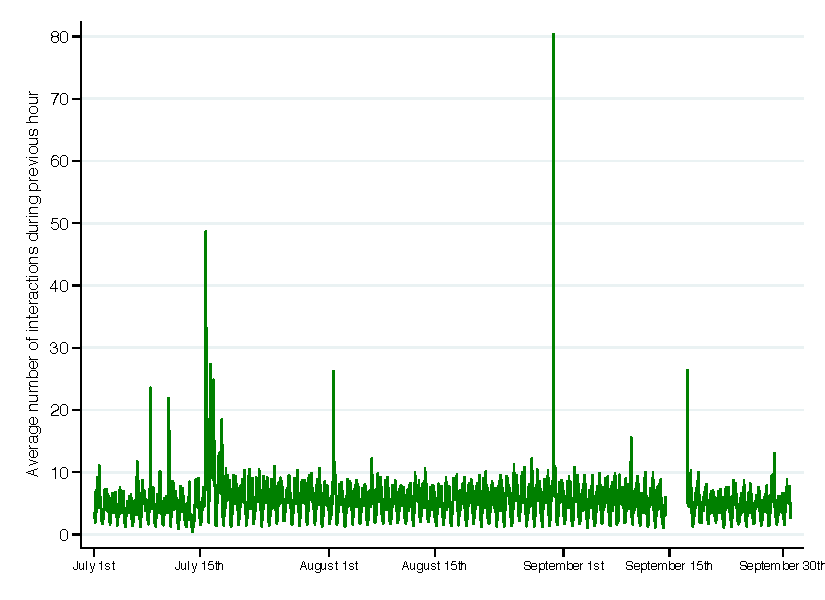
\includegraphics[scale=1]{figures/news_pressure_hour_illustration}
\end{center}
	\begin{spacing}{0.5}
		{\footnotesize \textbf{Notes:} The Figure reports the average number of interactions (retweets/replies/favorites) generated by the tweets published during the previous hour. The average number of interactions is computed at the minute-level.}
	\end{spacing}
\vspace{.5cm}	
	\caption{News pressure: Average number of interactions generated by the tweets published during the previous hour}
	\label{fig:news_pressure_hour_illustration}
\end{figure}
%%%%%%%%%%%%%%%%%%%%%%%%%%%%%%%%%%%%%%%%%%%%%%%%%%%%%%%%%%%%%%%%%%%%%% 

 
News pressure alone could not be a good instrument, however: it can indeed affect both Twitter and the media at the same time. It is why our instrument is the interaction between news pressure and the centrality in the network as previously defined. Our identification assumption is that, once we control for the direct effects of centrality and news pressure, the interaction between the seed's centrality and news pressure should only affect traditional news production through its effect on the tweet's visibility on Twitter. This is conditional on controlling for the seed's number of followers and, as highlighted above, dropping the events whose seed is the Twitter account of a media or of a journalist and/or whose seed is a multiple news breaker.



%%%%%%%%%%%%%%%%%%%%%%%%%%%%%%%%%%%%%%%%%%%%%%%%%%%%%%%%%%%%%%%%
%%%%%%%%%%%%%%%%%%%%%%%%%%%%%%%%%%%%%%%%%%%%%%%%%%%%%%%%%%%%%%%%
\section{Popularity on social media and news editors' decision: Results\label{Sec:Results}}
%%%%%%%%%%%%%%%%%%%%%%%%%%%%%%%%%%%%%%%%%%%%%%%%%%%%%%%%%%%%%%%%
%%%%%%%%%%%%%%%%%%%%%%%%%%%%%%%%%%%%%%%%%%%%%%%%%%%%%%%%%%%%%%%%

In this Section, we first present the results of the naive estimations (without instrumenting for the events popularity). We then turn to the IV analysis before discussing the heterogeneity of the effects.


%%%%%%%%%%%%%%%%%%%%%%%%%%%%%%%%%
\subsection{Naive estimates}

%%%%%%%%%%%%%%%%%%%%%%%%%%%%%%%%%
\paragraph{Event-level analysis}

Table \ref{Tab:number_articles_negbinomial_event} reports the results of the estimation of equation~(\ref{eq:OLSevent}) (event-level analysis). In Columns (1) to (4) the outcome of interest is total number of articles published in the event, and in Columns (5) and (6) the number of unique media outlets which cover the event. As highlighted above, given these dependent variables are count variables, we use a negative binomial. We find a positive correlation between the number of tweets published in an event before the first news article (``number of tweets") and the total number of articles published in the event: a $1,000$-increase in the number of tweets published in the event before the first media article is associated with $2.3$ additional articles (Column (1)); this finding is robust to dropping the events whose seed is the Twitter account of a media or of journalist and the events whose seed is Twitter account of a multiple news breaker (as defined above). Doing so only slightly decreases the magnitude of the relationship (Column (3)). Besides, this effect is mainly driven by the number of original tweets in the event; the number of retweets and replies do not have a positive effect (Columns (2) and (4)).

The positive relationship between the popularity of the event on Twitter and the media coverage is driven both by the intensity of the coverage (number of articles) and by the extensive margin: we also do find a positive relationship with the number of unique media outlets covering the event (Columns (5) and (6)). An increase by 1,000 in the number of original tweets published in the event before the first media article is associated with $1.3$ increase in the number of media outlets dealing with the event.


%%%%%%%%%%%%%%%%%%%%%%%%%%%%%%%%%%%%%%%%%%%%%%%%%%%%%%%%%%%%%%%%%%%%%%
\begin{table}
\caption{Naive estimates: Event-level approach}
\begin{center}
	{
\def\sym#1{\ifmmode^{#1}\else\(^{#1}\)\fi}
\begin{tabular}{l*{6}{c}}
\hline\hline
                    &\multicolumn{4}{c}{Number of articles}                                                 &\multicolumn{2}{c}{Number of media}        \\\cmidrule(lr){2-5}\cmidrule(lr){6-7}
                    &\multicolumn{1}{c}{(1)}         &\multicolumn{1}{c}{(2)}         &\multicolumn{1}{c}{(3)}         &\multicolumn{1}{c}{(4)}         &\multicolumn{1}{c}{(5)}         &\multicolumn{1}{c}{(6)}         \\
\hline
main                &                     &                     &                     &                     &                     &                     \\
Number of tweets    &       0.052\sym{***}&                     &       0.043\sym{***}&                     &       0.020\sym{***}&                     \\
                    &     (0.013)         &                     &     (0.010)         &                     &     (0.004)         &                     \\
Number of original tweets&                     &       0.517\sym{***}&                     &       0.394\sym{***}&                     &       0.079\sym{*}  \\
                    &                     &     (0.125)         &                     &     (0.132)         &                     &     (0.044)         \\
Number of retweets  &                     &      -0.005         &                     &       0.005         &                     &       0.016\sym{***}\\
                    &                     &     (0.009)         &                     &     (0.011)         &                     &     (0.006)         \\
Number of replies   &                     &      -0.331\sym{**} &                     &      -0.262\sym{*}  &                     &      -0.062         \\
                    &                     &     (0.161)         &                     &     (0.158)         &                     &     (0.092)         \\
Seed's number of followers&       0.000         &       0.000         &      -0.000         &      -0.000         &       0.000         &       0.000         \\
                    &     (0.000)         &     (0.000)         &     (0.000)         &     (0.000)         &     (0.000)         &     (0.000)         \\
\hline
Month \& DoW FEs    &  \checkmark         &  \checkmark         &  \checkmark         &  \checkmark         &  \checkmark         &  \checkmark         \\
Drop media          &                     &                     &  \checkmark         &  \checkmark         &  \checkmark         &  \checkmark         \\
Drop multiple       &                     &                     &  \checkmark         &  \checkmark         &  \checkmark         &  \checkmark         \\
Observations        &       4,259         &       4,259         &       3,163         &       3,163         &       3,163         &       3,163         \\
Marginal Effect (tweets)&         2.3         &                     &         1.8         &                     &         0.3         &                     \\
Marginal Effect (original tweets)&                     &        31.2         &                     &        18.2         &                     &         1.3         \\
\hline\hline
\end{tabular}
}

\end{center}
\begin{spacing}{0.5}
	{\fns \textbf{Notes:} * p$<$0.10, ** p$<$0.05, *** p$<$0.01. The time period is July 2018 - September 2018.  Models are estimated using a negative binomial estimation (robust standard errors are reported between parentheses). An observation is a news event. We only consider the subset of news events that appear first on Twitter. All specifications include the seed's number of followers as a control, and day-of-the-week and month fixed effects. Columns (1) and (2) report the estimates for all the events that appear first on Twitter; in Columns (3) to (6) we drop the events whose seed is the Twitter account of a media or of journalist (``media") as well as the events whose seed broke more than one event during our time period (``multiple"). The independent variables (number of tweets, number of original tweets, etc.) are computed \textit{before} the first news article in the event and are in thousand. More details are provided in the text.} 
\end{spacing}
\label{Tab:number_articles_negbinomial_event}
\end{table} 
%%%%%%%%%%%%%%%%%%%%%%%%%%%%%%%%%%%%%%%%%%%%%%%%%%%%%%%%%%%%%%%%%%%%%%


%%%%%%%%%%%%%%%%%%%%%%%%%%%%%%%%%
\paragraph{Media-level analysis}

Table \ref{Tab:number_articles_negbinomial_cevent} shows the estimates when we perform the media-level analysis (estimation of equation~(\ref{eq:OLSmedia})). The unit of observation is a media-event, and all the media outlets are included in the estimation (even if they do not cover the event; then the value of the number of articles in the event for them is equal to zero). Consistently with the results in Table \ref{Tab:number_articles_negbinomial_event}, we find a positive relationship between the popularity of the event on Twitter and the media coverage it receives (Column (1)), and this relationship is robust to dropping the events whose seed is the Twitter account of a media / journalist / multiple news breaker (Column (2)). A $1,000$-increase in the number of tweets published in the event before the first media article increases the average number of articles \textit{each media outlet} publishes in the event by $0.011$. 

In Columns (3) to (6) we investigate whether this relationship varies with the media characteristics, and in particular with the intensity of their social media presence. We define this intensity here with respect to the share of the media outlet's articles that are published on social media. We find that the strength of the relationship is higher for the outlets whose social media presence is high than for the media whose social media presence is relatively lower. We will come back to this finding when discussing the mechanisms at play in Section \ref{Sec:Mechanisms} below. We then investigate whether these effects depend on the offline format of the media. Table \ref{Tab:number_articles_negbinomial_cevent_heterogeneity} presents the results. While we observe a positive and statistically significant relationship for all the media outlets, the magnitude is the strongest for the websites of the television stations.
% JULIA: A RAJOUTER PLUS TARD Robustness avec les autres mesures de social media presence (e.g. number of Twitter accounts)


%%%%%%%%%%%%%%%%%%%%%%%%%%%%%%%%%%%%%%%%%%%%%%%%%%%%%%%%%%%%%%%%%%%%%%
\begin{sidewaystable}
\caption{Naive estimates: Media-level approach}
\begin{center}
	{
\def\sym#1{\ifmmode^{#1}\else\(^{#1}\)\fi}
\begin{tabular}{l*{6}{c}}
\hline\hline
                    &\multicolumn{2}{c}{All}                    &\multicolumn{2}{c}{Low social media presence}&\multicolumn{2}{c}{High social media presence}\\\cmidrule(lr){2-3}\cmidrule(lr){4-5}\cmidrule(lr){6-7}
                    &\multicolumn{1}{c}{(1)}         &\multicolumn{1}{c}{(2)}         &\multicolumn{1}{c}{(3)}         &\multicolumn{1}{c}{(4)}         &\multicolumn{1}{c}{(5)}         &\multicolumn{1}{c}{(6)}         \\
\hline
Number of articles  &                     &                     &                     &                     &                     &                     \\
Number of tweets    &       0.048\sym{***}&       0.041\sym{***}&       0.042\sym{***}&       0.038\sym{***}&       0.050\sym{***}&       0.042\sym{***}\\
                    &     (0.009)         &     (0.008)         &     (0.009)         &     (0.008)         &     (0.010)         &     (0.008)         \\
Seed's number of followers&       0.000         &      -0.000         &       0.000\sym{*}  &      -0.000         &       0.000         &      -0.000         \\
                    &     (0.000)         &     (0.000)         &     (0.000)         &     (0.000)         &     (0.000)         &     (0.000)         \\
\hline
Media FEs           &  \checkmark         &  \checkmark         &  \checkmark         &  \checkmark         &  \checkmark         &  \checkmark         \\
Month \& DoW FEs    &  \checkmark         &  \checkmark         &  \checkmark         &  \checkmark         &  \checkmark         &  \checkmark         \\
Drop media          &                     &  \checkmark         &                     &  \checkmark         &                     &  \checkmark         \\
Drop multiple       &                     &  \checkmark         &                     &  \checkmark         &                     &  \checkmark         \\
Observations        &     800,692         &     594,644         &     400,346         &     297,322         &     400,346         &     297,322         \\
Clusters (events)   &       4,259         &       3,163         &       4,259         &       3,163         &       4,259         &       3,163         \\
Marginal Effect     & {0.011}             &     0.009           & {0.007}             &       0.006         & {0.015}             &       0.012        \\
\hline\hline
\end{tabular}
}

\end{center}
\begin{spacing}{0.5}
	{\fns \textbf{Notes:} * p$<$0.10, ** p$<$0.05, *** p$<$0.01. The time period is July 2018 - September 2018.  Models are estimated using a negative binomial estimation. Standard errors are clustered at the event level. An observation is a media-news event. We only consider the subset of news events that appear first on Twitter. All specifications include the seed's number of followers as a control, and day-of-the-week, month, and media fixed effects. Columns (1), (3) and (5) report the estimates for all the events that appear first on Twitter; in Columns (2), (4) and (6) we drop the events whose seed is the Twitter account of a media or of journalist (``media") as well as the events whose seed broke more than one event during our time period (``multiple"). In Columns (1) and (2) all the media outlets in our sample are included; in Columns (3) and (4) (respectively Columns (5) and (6)) we only consider the media outlets whose social media presence is low (respectively high). High and low social media presence are defined by the share of the media outlet's articles published on social media (above or below the median). The number of tweets is computed \textit{before} the first news article in the event and is in thousand. More details are provided in the text.} 
\end{spacing}
\label{Tab:number_articles_negbinomial_cevent}
\end{sidewaystable} 
%%%%%%%%%%%%%%%%%%%%%%%%%%%%%%%%%%%%%%%%%%%%%%%%%%%%%%%%%%%%%%%%%%%%%%


%%%%%%%%%%%%%%%%%%%%%%%%%%%%%%%%%%%%%%%%%%%%%%%%%%%%%%%%%%%%%%%%%%%%%%
\begin{table}
\caption{Naive estimates: Media-level approach, Depending on the media offline format}
\begin{center}
	{
\def\sym#1{\ifmmode^{#1}\else\(^{#1}\)\fi}
\begin{tabular}{l*{6}{c}}
\hline\hline
                    &\multicolumn{1}{c}{Nat. dail.}&\multicolumn{1}{c}{Local dail.}&\multicolumn{1}{c}{Weeklies}&\multicolumn{1}{c}{Pure online}&\multicolumn{1}{c}{TV}&\multicolumn{1}{c}{Radio}\\\cmidrule(lr){2-2}\cmidrule(lr){3-3}\cmidrule(lr){4-4}\cmidrule(lr){5-5}\cmidrule(lr){6-6}\cmidrule(lr){7-7}
                    &\multicolumn{1}{c}{(1)}         &\multicolumn{1}{c}{(2)}         &\multicolumn{1}{c}{(3)}         &\multicolumn{1}{c}{(4)}         &\multicolumn{1}{c}{(5)}         &\multicolumn{1}{c}{(6)}         \\
\hline
Number of articles  &                     &                     &                     &                     &                     &                     \\
Number of tweets    &       0.033\sym{***}&       0.039\sym{***}&       0.042\sym{***}&       0.048\sym{***}&       0.059\sym{***}&       0.039\sym{***}\\
                    &     (0.009)         &     (0.008)         &     (0.008)         &     (0.009)         &     (0.013)         &     (0.009)         \\
Seed's number of followers&      -0.000\sym{**} &      -0.000         &      -0.000         &       0.000         &      -0.000         &      -0.000         \\
                    &     (0.000)         &     (0.000)         &     (0.000)         &     (0.000)         &     (0.000)         &     (0.000)         \\
\hline
Media FEs           &  \checkmark         &  \checkmark         &  \checkmark         &  \checkmark         &  \checkmark         &  \checkmark         \\
Month \& DoW FEs    &  \checkmark         &  \checkmark         &  \checkmark         &  \checkmark         &  \checkmark         &  \checkmark         \\
Drop media          &  \checkmark         &  \checkmark         &  \checkmark         &  \checkmark         &  \checkmark         &  \checkmark         \\
Drop multiple       &  \checkmark         &  \checkmark         &  \checkmark         &  \checkmark         &  \checkmark         &  \checkmark         \\
Observations        &      34,793         &      88,564         &     107,542         &     205,595         &      22,141         &      34,793         \\
Clusters (events)   &       3,163         &       3,163         &       3,163         &       3,163         &       3,163         &       3,163         \\
Marginal Effect     &       0.017         &       0.012         &       0.009         &       0.003         &       0.020         &       0.013         \\
\hline\hline
\end{tabular}
}

\end{center}
\begin{spacing}{0.5}
	{\fns \textbf{Notes:} * p$<$0.10, ** p$<$0.05, *** p$<$0.01. The time period is July 2018 - September 2018.  Models are estimated using a negative binomial estimation. Standard errors are clustered at the event level. An observation is a media-news event. We only consider the subset of news events that appear first on Twitter, and drop the events whose seed is the Twitter account of a media or of journalist (``media") as well as the events whose seed broke more than one event during our time period (``multiple"). All specifications include the seed's number of followers as a control, and day-of-the-week, month, and media fixed effects. In Column (1), we only consider the national daily newspapers, in Column (2) the local daily newspapers, in Column (3) the weekly newspapers, in Column (4) the pure online media, in Column (5) the websites of the television stations, and in Column (6) the websites of the radio channels. The number of tweets is computed \textit{before} the first news article in the event and is in thousand. More details are provided in the text.} 
\end{spacing}
\label{Tab:number_articles_negbinomial_cevent_heterogeneity}
\end{table} 
%%%%%%%%%%%%%%%%%%%%%%%%%%%%%%%%%%%%%%%%%%%%%%%%%%%%%%%%%%%%%%%%%%%%%%


%%%%%%%%%%%%%%%%%%%%%%%%%%%%%%%%%%%%%%%%%%%%%%%%%%%%%%%%%%%%%%%%%%%%%
% POUR L'INSTANT ON NE MONTRE PAS CETTE TABLE -- PEUT-ETRE APRES L'IV
%\begin{sidewaystable}
%\caption{Naive estimates: Media-level approach, Depending on the offline format}
%\begin{center}
%	{
\def\sym#1{\ifmmode^{#1}\else\(^{#1}\)\fi}
\begin{tabular}{l*{8}{c}}
\hline\hline
                    &\multicolumn{2}{c}{No paywall}             &\multicolumn{2}{c}{Paywall}                &\multicolumn{2}{c}{Small newsroom}         &\multicolumn{2}{c}{Large newsroom}         \\\cmidrule(lr){2-3}\cmidrule(lr){4-5}\cmidrule(lr){6-7}\cmidrule(lr){8-9}
                    &\multicolumn{1}{c}{(1)}         &\multicolumn{1}{c}{(2)}         &\multicolumn{1}{c}{(3)}         &\multicolumn{1}{c}{(4)}         &\multicolumn{1}{c}{(5)}         &\multicolumn{1}{c}{(6)}         &\multicolumn{1}{c}{(7)}         &\multicolumn{1}{c}{(8)}         \\
\hline
Number of articles  &                     &                     &                     &                     &                     &                     &                     &                     \\
Number of tweets    &       0.051\sym{***}&       0.045\sym{***}&       0.044\sym{***}&       0.036\sym{***}&       0.044\sym{***}&       0.038\sym{***}&       0.052\sym{***}&       0.041\sym{***}\\
                    &     (0.008)         &     (0.008)         &     (0.011)         &     (0.008)         &     (0.010)         &     (0.009)         &     (0.013)         &     (0.009)         \\
Seed's number of followers&       0.000         &       0.000         &       0.000         &      -0.000\sym{*}  &       0.000\sym{*}  &      -0.000         &       0.000\sym{*}  &      -0.000         \\
                    &     (0.000)         &     (0.000)         &     (0.000)         &     (0.000)         &     (0.000)         &     (0.000)         &     (0.000)         &     (0.000)         \\
\hline
Media FEs           &  \checkmark         &  \checkmark         &  \checkmark         &  \checkmark         &  \checkmark         &  \checkmark         &  \checkmark         &  \checkmark         \\
Month \& DoW FEs    &  \checkmark         &  \checkmark         &  \checkmark         &  \checkmark         &  \checkmark         &  \checkmark         &  \checkmark         &  \checkmark         \\
Drop media          &                     &  \checkmark         &                     &  \checkmark         &                     &  \checkmark         &                     &  \checkmark         \\
Drop multiple       &                     &  \checkmark         &                     &  \checkmark         &                     &  \checkmark         &                     &  \checkmark         \\
Observations        &     472,749         &     351,093         &     264,058         &     196,106         &     140,547         &     104,379         &     144,806         &     107,542         \\
Clusters (events)   &       4,259         &       3,163         &       4,259         &       3,163         &       4,259         &       3,163         &       4,259         &       3,163         \\
Marginal Effect     &       0.011         &       0.010         &       0.013         &       0.010         &       0.010         &       0.008         &       0.047         &       0.034         \\
\hline\hline
\end{tabular}
}

%\end{center}
%\begin{spacing}{0.5}
%	{\fns \textbf{Notes:} \textbf{REPRENDRE}} 
%\end{spacing}
%\label{Tab:number_articles_negbinomial_cevent_heterogeneity_paywall_journalists}
%\end{sidewaystable} 
%%%%%%%%%%%%%%%%%%%%%%%%%%%%%%%%%%%%%%%%%%%%%%%%%%%%%%%%%%%%%%%%%%%%%%


Next, we focus on the media outlets that devote at least one article to the event and investigate the magnitude of the coverage, \textit{conditional on covering} the event. Indeed, the popularity of an event on Twitter can indeed play a role both at the intensive and at the extensive margin. Table \ref{Tab:number_articles_negbinomial_Dcover_cevent} presents the results. Columns (1) and (2) present the estimations for the number of articles published by the media in the event: we see that the positive impact of popularity appears not only at the extensive margin but also at the intensive margin given there is a positive correlation with the number of articles published (conditional on publishing at least one article in the event). However, the magnitude of this relationship is weak: a $1,000$-increase in the the number of tweets is associated with an increase in the number of articles published by each media outlet by $0.05$.

Besides, we find a statistically significant relationship with the length of the article(s) published by the media (Columns (3) and (4)). While an imperfect one, the length of the articles can be considered as a proxy for the quality of the articles. We will come back to this point in the mechanisms section below.


%%%%%%%%%%%%%%%%%%%%%%%%%%%%%%%%%%%%%%%%%%%%%%%%%%%%%%%%%%%%%%%%%%%%%%
\begin{table}
\caption{Naive estimates: Media-level approach, Conditional on covering the event}
\begin{center}
	{
\def\sym#1{\ifmmode^{#1}\else\(^{#1}\)\fi}
\begin{tabular}{l*{4}{c}}
\hline\hline
                    &\multicolumn{2}{c}{Number of articles}     &\multicolumn{2}{c}{Articles length}        \\\cmidrule(lr){2-3}\cmidrule(lr){4-5}
                    &\multicolumn{1}{c}{(1)}         &\multicolumn{1}{c}{(2)}         &\multicolumn{1}{c}{(3)}         &\multicolumn{1}{c}{(4)}         \\
\hline
main                &                     &                     &                     &                     \\
Number of tweets    &        0.02\sym{***}&        0.02\sym{***}&        7.58\sym{***}&        7.64\sym{***}\\
                    &      (0.01)         &      (0.00)         &      (2.38)         &      (2.51)         \\
Seed's number of followers&        0.00         &       -0.00\sym{*}  &        0.00         &       -0.00         \\
                    &      (0.00)         &      (0.00)         &      (0.00)         &      (0.00)         \\
\hline
Media FEs           &  \checkmark         &  \checkmark         &  \checkmark         &  \checkmark         \\
Month \& DoW FEs    &  \checkmark         &  \checkmark         &  \checkmark         &  \checkmark         \\
Drop media          &                     &  \checkmark         &                     &  \checkmark         \\
Drop multiple       &                     &  \checkmark         &                     &  \checkmark         \\
R-sq (within)       &                     &                     &       0.001         &       0.001         \\
Observations        &      70,133         &      52,246         &      70,124         &      52,237         \\
Clusters (events)   &       4,259         &       3,163         &       4,259         &       3,163         \\
Marginal Effect     &        0.05         &        0.04         &                     &                     \\
\hline\hline
\end{tabular}
}

\end{center}
\begin{spacing}{0.5}
	{\fns \textbf{Notes:} * p$<$0.10, ** p$<$0.05, *** p$<$0.01. The time period is July 2018 - September 2018.  Models are estimated using a negative binomial estimation in Columns (1) and (2), and OLS in Columns (3) to (4). Standard errors are clustered at the event level. An observation is a media-news event, and only the media outlets that devote at least one article to the event are included. Further, we only consider the subset of news events that appear first on Twitter. All specifications include the seed's number of followers as a control, and day-of-the-week, month, and media fixed effects. Columns (1) and (3) report the estimates for all the events that appear first on Twitter; in Columns (2) and (4) we drop the events whose seed is the Twitter account of a media or of journalist (``media") as well as the events whose seed broke more than one event during our time period (``multiple"). In Columns (1) and (2), the dependent variable is the number of articles published by the media outlet; in Columns (3) and (4) the average length of these articles. The number of tweets is computed \textit{before} the first news article in the event and is in thousand. More details are provided in the text.}
% , and in Columns (5) and (6) the reaction time in hour (we take the minimum reaction time when the media publishes more than one article in the event)	
\end{spacing}
\label{Tab:number_articles_negbinomial_Dcover_cevent}
\end{table} 
%%%%%%%%%%%%%%%%%%%%%%%%%%%%%%%%%%%%%%%%%%%%%%%%%%%%%%%%%%%%%%%%%%%%%%



%%%%%%%%%%%%%%%%%%%%%%%%%%%%%%%%%
\subsection{IV estimates\label{Sec:ResultsIV}}
%%%%%%%%%%%%%%%%%%%%%%%%%%%%%%%%%

The previous estimates may suffer from the fact that the positive relationship between a story popularity on Twitter and its media coverage can both be driven by the intrinsic interest of the story, independently of what happens on social media. Hence, in this section, we report the results of the IV estimates following the strategy described in Section \ref{Sec:SpecificationIV} above.

Table \ref{Tab:number_articles_IV} reports the results of the estimation. In Columns (1) and (2) we report the results of the first stage (the dependent variable is the number of tweets before the number of articles in the event) and in Columns (3) and (4) the second, where the main explanatory variable, number of tweets, is instrumented by the interaction between news pressure and the centrality in the network. As appears clearly from Columns (1) and (2), our instrument ``High pressure * Previous interactions" has a statistically significant effect on the number of tweets in the event. Second, we find that there is a positive and statistically significant causal effect of the number of tweets on the number of articles (Columns (3) and (4)). This effect is robust to dropping the events whose seed is the Twitter account of a media / journalist / multiple news breaker (as previously defined).

Regarding the magnitude of the effects, we find that a $1,000$ increase in the number of tweets is associated with an increase by $1.11$ in the number of articles published in the event. Hence the magnitude of the IV estimates is around half the one of the naive estimates. This is consistent with the expected direction of the bias given the unobserved newsworthiness of events should drive upward both the number of articles and the number of tweets in the event.


%%%%%%%%%%%%%%%%%%%%%%%%%%%%%%%%%%%%%%%%%%%%%%%%%%%%%%%%%%%%%%%%%%%%%%
\begin{table}
\caption{IV estimates: Media-level approach}
\begin{center}
	{
\def\sym#1{\ifmmode^{#1}\else\(^{#1}\)\fi}
\begin{tabular}{l*{4}{c}}
\hline\hline
                    &\multicolumn{2}{c}{Number of tweets}       &\multicolumn{2}{c}{Number of articles}     \\\cmidrule(lr){2-3}\cmidrule(lr){4-5}
                    &\multicolumn{1}{c}{(1)}         &\multicolumn{1}{c}{(2)}         &\multicolumn{1}{c}{(3)}         &\multicolumn{1}{c}{(4)}         \\
\hline
\textbf{Instrument} &                     &                     &                     &                     \\
High pressure * Previous interactions&      -0.015\sym{***}&-0.016\sym{***}&                     &                     \\
                    &     (0.000)         &     (0.000)         &                     &                     \\
\textbf{Controls}   &                     &                     &                     &                     \\
Previous interactions&       0.016\sym{***}&0.016\sym{***}&-0.249\sym{***}&      -0.023\sym{***}\\
                    &     (0.000)         &     (0.000)         &     (0.000)         &     (0.000)         \\
High pressure       &      -0.061\sym{***}&-0.068\sym{***}&       2.250\sym{***}&      -0.958\sym{***}\\
                    &     (0.000)         &     (0.000)         &     (0.000)         &     (0.000)         \\
Seed's followers (thsd)&      -0.000\sym{***}&       0.000\sym{***}&       0.000\sym{***}&       0.000\sym{***}\\
                    &     (0.000)         &     (0.000)         &     (0.000)         &     (0.000)         \\
\textbf{Second stage}&                     &                     &                     &                     \\
Nb of tweets        &                     &                     &      12.814\sym{***}&1.110\sym{***}\\
                    &                     &                     &     (0.000)         &     (0.000)         \\
\hline
Media FEs           &    \checkmark       &     \checkmark      &  \checkmark         &  \checkmark         \\
Month \& DoW FEs    &    \checkmark       &     \checkmark      &  \checkmark         &  \checkmark         \\
Drop media          &                     &     \checkmark      &                     &  \checkmark         \\
Drop multiple       &                     &     \checkmark      &                     &  \checkmark         \\
Observations        &     792,984         &     586,936         &     792,984         &     586,936         \\
Underidentification (p-value)&                     &                     &        0.00         &        0.00         \\
Mean DepVar         &                     &                     &       43.19         &       41.19         \\
Sd DepVar           &                     &                     &       89.97         &       76.81         \\
\hline\hline
\end{tabular}
}

\end{center}
\begin{spacing}{0.5}
	{\fns \textbf{Notes:} * p$<$0.10, ** p$<$0.05, *** p$<$0.01. The time period is July 2018 - September 2018.  An observation is a media-news event. Standard errors are clustered at the event level. All specifications include the seed's number of followers as a control, and day-of-the-week, month, and media fixed effects. Columns (1) and (2) report the results of the first stage and Columns (3) and (4) of the second stage. In Columns (2) and (4) we drop the events whose seed is the Twitter account of a media or of journalist (``media") as well as the events whose seed broke more than one event during our time period (``multiple"). The number of tweets is computed \textit{before} the first news article in the event and is in thousand. More details are provided in the text.}
\end{spacing}
\label{Tab:number_articles_IV}
\end{table} 
%%%%%%%%%%%%%%%%%%%%%%%%%%%%%%%%%%%%%%%%%%%%%%%%%%%%%%%%%%%%%%%%%%%%%%


Last, we investigate the causal effect of the popularity on Twitter at the extensive margin and focus as before on the media outlets that devote at least one article to the event. Table \ref{Tab:number_articles_IV_Dcover} presents our results. Consistently with the findings of Table \ref{Tab:number_articles_IV}, we show that our effects are robust to instrumenting for the popularity of events on Twitter, and that the magnitude of the IV estimates is lower than the one of the naive estimates.


%%%%%%%%%%%%%%%%%%%%%%%%%%%%%%%%%%%%%%%%%%%%%%%%%%%%%%%%%%%%%%%%%%%%%%
\begin{table}
\caption{IV estimates: Media-level approach, Conditional on covering the event}
\begin{center}
	{
\def\sym#1{\ifmmode^{#1}\else\(^{#1}\)\fi}
\begin{tabular}{l*{4}{c}}
\hline\hline
                    &\multicolumn{2}{c}{Number of articles}     &\multicolumn{2}{c}{Articles length}        \\\cmidrule(lr){2-3}\cmidrule(lr){4-5}
                    &\multicolumn{1}{c}{(1)}         &\multicolumn{1}{c}{(2)}         &\multicolumn{1}{c}{(3)}         &\multicolumn{1}{c}{(4)}         \\
\hline
\textbf{Second stage}&                     &                     &                     &                     \\
Nb of tweets        &       0.310\sym{***}&      11.835\sym{***}&      83.624\sym{*}  &      11.835\sym{***}\\
                    &     (0.120)         &     (2.073)         &    (45.284)         &     (2.073)         \\
\textbf{Controls}   &                     &                     &                     &                     \\
Previous interactions&      -0.008\sym{***}&      -0.260\sym{***}&      -1.648\sym{**} &      -0.260\sym{***}\\
                    &     (0.002)         &     (0.042)         &     (0.820)         &     (0.042)         \\
High pressure       &       0.104\sym{***}&      -2.711\sym{***}&      -3.807         &      -2.711\sym{***}\\
                    &     (0.027)         &     (0.817)         &    (17.297)         &     (0.817)         \\
Seed's followers (thsd)&       0.000\sym{***}&       0.000\sym{***}&       0.000\sym{***}&       0.000\sym{***}\\
                    &     (0.000)         &     (0.000)         &     (0.000)         &     (0.000)         \\
\hline
Media FEs           &  \checkmark         &  \checkmark         &  \checkmark         &  \checkmark         \\
Month \& DoW FEs    &  \checkmark         &  \checkmark         &  \checkmark         &  \checkmark         \\
Drop media          &                     &  \checkmark         &                     &  \checkmark         \\
Drop multiple       &                     &  \checkmark         &                     &  \checkmark         \\
Observations        &      69,466         &      51,579         &      69,466         &      51,579         \\
Underidentification (p-value)&        0.00         &        0.00         &        0.00         &        0.00         \\
Mean DepVar         &        2.62         &       75.92         &    2,540.71         &       75.92         \\
Sd DepVar           &        6.51         &      129.41         &    1,607.70         &      129.41         \\
\hline\hline
\end{tabular}
}

\end{center}
\begin{spacing}{0.5}
	{\fns \textbf{Notes:} * p$<$0.10, ** p$<$0.05, *** p$<$0.01. The time period is July 2018 - September 2018.  An observation is a media-news event. Standard errors are clustered at the event level. All specifications include the seed's number of followers as a control, and day-of-the-week, month, and media fixed effects. Columns (1) and (2) report the results of the first stage and Columns (3) and (4) of the second stage. In Columns (2) and (4) we drop the events whose seed is the Twitter account of a media or of journalist (``media") as well as the events whose seed broke more than one event during our time period (``multiple"). The number of tweets is computed \textit{before} the first news article in the event and is in thousand. More details are provided in the text.}
\end{spacing}
\label{Tab:number_articles_IV_Dcover}
\end{table} 
%%%%%%%%%%%%%%




%%%%%%%%%%%%%%%%%%%%%%%%%%%%%%%%%%%%%%%%%%%%%%%%%%%%%%%%%%%%%%%%
%%%%%%%%%%%%%%%%%%%%%%%%%%%%%%%%%%%%%%%%%%%%%%%%%%%%%%%%%%%%%%%%
\section{Mechanisms\label{Sec:Mechanisms}}
In the previous section, we have documented a positive relationship between the popularity of an event on Twitter and the coverage it receives on mainstream media. In this section, we discuss the different mechanisms at play behind this relationship.
% , and show that this relationship can be interpreted as causal

%%%%%%%%%%%%%%%%%%%%%%%%%%%%%%%%%
\subsection{Journalists monitor Twitter}
%%%%%%%%%%%%%%%%%%%%%%%%%%%%%%%%%

First of all, the fact that a number of stories appear first on Twitter and that we observe high reactivity of the mainstream media might be due to the fact that journalists are closely monitoring Twitter. A growing literature in journalism studies indeed highlights that social media play an important role as a news source. For example, \citet{vonNordheimBoczekKoppers2018} examine the use of Facebook and Twitter as journalistic sources in newspapers of three countries; they show that Twitter is more commonly used as a news source than Facebook.\footnote{For additional evidence of Twitter as a reporting tool, see e.g. \citet{Vis2012}.} Further, \citet{McGregorMolyneux2018}, who have conducted an online survey experiment on working U.S. journalists, show that journalists using Twitter as part of their daily work consider tweets as newsworthy as headlines from the Associated Press.

The use of Twitter crosses many dimensions of sourcing, information-gathering, and production of stories \citep{Wihbeyetal2018}. Most media organizations actively encourage journalistic activity on social media.   Among the $4,222,734$ Twitter accounts for which we have data, $0.12\%$ are the accounts of journalists (see Table \ref{Tab:table_summary_users_all_first} above); while this might seem low, it is actually rather high compared to the share of the total adult population journalists represent.

To investigate the role played by monitoring, for all the media organizations included in our sample, we compute the list of their journalists present on Twitter, and investigate the heterogeneity of the effects depending on this variable. Table \ref{Tab:number_articles_negbinomial_cevent_heterogeneity_nb_journalist_accounts} reports the results. While the coefficient on the effect of the number of tweets on the media coverage is pretty much similar for the media that have a high number of journalists with a Twitter account (Columns (3) and (4)) than for those with only a few numbers (Columns (1) and (2)), the marginal effect is twice as high for the former. Hence, while it cannot entirely explain our findings, the monitoring of Twitter by journalists seems to play a role here.


%%%%%%%%%%%%%%%%%%%%%%%%%%%%%%%%%%%%%%%%%%%%%%%%%%%%%%%%%%%%%%%%%%%%%%
\begin{table}
\caption{Naive estimates: Media-level approach, Depending on the number of journalists with a Twitter account}
\begin{center}
	{
\def\sym#1{\ifmmode^{#1}\else\(^{#1}\)\fi}
\begin{tabular}{l*{4}{c}}
\hline\hline
                    &\multicolumn{2}{c}{Low no. of journalists with Twitter}&\multicolumn{2}{c}{High no. of journalists with Twitter}\\\cmidrule(lr){2-3}\cmidrule(lr){4-5}
                    &\multicolumn{1}{c}{(1)}         &\multicolumn{1}{c}{(2)}         &\multicolumn{1}{c}{(3)}         &\multicolumn{1}{c}{(4)}         \\
\hline
Number of articles  &                     &                     &                     &                     \\
Number of tweets    &       0.044\sym{***}&       0.038\sym{***}&       0.046\sym{***}&       0.039\sym{***}\\
                    &     (0.010)         &     (0.009)         &     (0.010)         &     (0.008)         \\
Seed's number of followers&       0.000         &      -0.000         &       0.000         &      -0.000         \\
                    &     (0.000)         &     (0.000)         &     (0.000)         &     (0.000)         \\
\hline
Media FEs           &  \checkmark         &  \checkmark         &  \checkmark         &  \checkmark         \\
Month \& DoW FEs    &  \checkmark         &  \checkmark         &  \checkmark         &  \checkmark         \\
Drop media          &                     &  \checkmark         &                     &  \checkmark         \\
Drop multiple       &                     &  \checkmark         &                     &  \checkmark         \\
Observations        &     127,770         &      94,890         &     383,310         &     284,670         \\
Clusters (events)   &       4,259         &       3,163         &       4,259         &       3,163         \\
Marginal Effect     &       0.010         &  \emph{0.008}       &       0.019         &  \emph{0.015}       \\
\hline\hline
\end{tabular}
}

\end{center}
\begin{spacing}{0.5}
	{\fns \textbf{Notes:} * p$<$0.10, ** p$<$0.05, *** p$<$0.01. The time period is July 2018 - September 2018. Models are estimated using a negative binomial estimation. Standard errors are clustered at the event level. An observation is a media-news event.  Columns (1) and (3) report the estimates for all the events that appear first on Twitter; in Columns (2) and (4)  we drop the events whose seed is the Twitter account of a media or of journalist (``media") as well as the events whose seed broke more than one event during our time period (``multiple"). All specifications include the seed's number of followers as a control, and day-of-the-week, month, and media fixed effects. In Columns (1) and (2) (respectively (3) and (4), we consider the media with a relatively low (respectively relatively high) number of journalists with a Twitter account. The number of tweets is computed \textit{before} the first news article in the event and is in thousand. More details are provided in the text.} 
\end{spacing}
\label{Tab:number_articles_negbinomial_cevent_heterogeneity_nb_journalist_accounts}
\end{table} 
%%%%%%%%%%%%%%%%%%%%%%%%%%%%%%%%%%%%%%%%%%%%%%%%%%%%%%%%%%%%%%%%%%%%%%

%However, this explains the relationship we observe on the extensive margin, but not on the intensive margin.


%\begin{center}
%\textbf{[TO BE COMPLETED]}
%\end{center}
%
%
%To see role played by social media, we also investigate media outlets' strategy on Twitter: in particular, how many times they tweet in the event. \textbf{TO BE DONE}



%%%%%%%%%%%%%%%%%%%%%%%%%%%%%%%%%
\subsection{Editorial decisions and popularity}
%%%%%%%%%%%%%%%%%%%%%%%%%%%%%%%%%
% Clicks bias or Signaling model?

The causal relationship between the popularity of a story on Twitter and its mainstream media coverage can be due do the existence of a clicks bias. This explanation is consistent with the results of \citet{SenYildirim2015} that show, using data from a leading English language Indian national daily newspaper, that editors' coverage decisions of online news stories are influenced by the observed popularity of the story, as measured by the number of clicks received.

In \citet{SenYildirim2015}'s framework (that builds on \citet{Latham2015}), the newspaper cares about the revenue generated by covering a story, which is assumed to be proportional to the number of readers. To test for this hypothesis here, we use the fact that our sample of media outlets include a lot of different media outlets, some of them relying on advertising revenues while others do not. Table \ref{Tab:number_articles_negbinomial_cevent_heterogeneity_advertising} presents our estimates depending on whether the media rely on advertising revenues (around 80\% of the media outlets in our sample do so). The order of magnitude of the estimated effects of popularity on Twitter on media coverage is more or less similar in both cases; if anything, the marginal effects are slightly higher for the media that do not rely on advertising online.


%%%%%%%%%%%%%%%%%%%%%%%%%%%%%%%%%%%%%%%%%%%%%%%%%%%%%%%%%%%%%%%%%%%%
\begin{table}
\caption{Naive estimates: Media-level approach, Depending on the reliance on advertising revenues}
\begin{center}
	{
\def\sym#1{\ifmmode^{#1}\else\(^{#1}\)\fi}
\begin{tabular}{l*{4}{c}}
\hline\hline
                    &\multicolumn{2}{c}{No advertising}         &\multicolumn{2}{c}{Advertising}            \\\cmidrule(lr){2-3}\cmidrule(lr){4-5}
                    &\multicolumn{1}{c}{(1)}         &\multicolumn{1}{c}{(2)}         &\multicolumn{1}{c}{(3)}         &\multicolumn{1}{c}{(4)}         \\
\hline
Number of articles  &                     &                     &                     &                     \\
Number of tweets    &       0.049\sym{***}&       0.044\sym{***}&       0.048\sym{***}&       0.041\sym{***}\\
                    &     (0.010)         &     (0.011)         &     (0.009)         &     (0.007)         \\
Seed's number of followers&       0.000\sym{*}  &      -0.000\sym{**} &       0.000         &      -0.000         \\
                    &     (0.000)         &     (0.000)         &     (0.000)         &     (0.000)         \\
\hline
Media FEs           &  \checkmark         &  \checkmark         &  \checkmark         &  \checkmark         \\
Month \& DoW FEs    &  \checkmark         &  \checkmark         &  \checkmark         &  \checkmark         \\
Drop media          &                     &  \checkmark         &                     &  \checkmark         \\
Drop multiple       &                     &  \checkmark         &                     &  \checkmark         \\
Observations        &     140,547         &     104,379         &     596,260         &     442,820         \\
Clusters (events)   &       4,259         &       3,163         &       4,259         &       3,163         \\
Marginal Effect     &       0.017         &       0.014         &       0.011         &       0.009         \\
\hline\hline
\end{tabular}
}

\end{center}
\begin{spacing}{0.5}
	{\fns \textbf{Notes:} * p$<$0.10, ** p$<$0.05, *** p$<$0.01. The time period is July 2018 - September 2018. Models are estimated using a negative binomial estimation. Standard errors are clustered at the event level. An observation is a media-news event.  Columns (1) and (3) report the estimates for all the events that appear first on Twitter; in Columns (2) and (4)  we drop the events whose seed is the Twitter account of a media or of journalist (``media") as well as the events whose seed broke more than one event during our time period (``multiple"). All specifications include the seed's number of followers as a control, and day-of-the-week, month, and media fixed effects. In Columns (1) and (2) (respectively (3) and (4), we consider the media without online advertising (respectively with advertising revenues). The number of tweets is computed \textit{before} the first news article in the event and is in thousand. More details are provided in the text.} 
\end{spacing}
\label{Tab:number_articles_negbinomial_cevent_heterogeneity_advertising}
\end{table} 
%%%%%%%%%%%%%%%%%%%%%%%%%%%%%%%%%%%%%%%%%%%%%%%%%%%%%%%%%%%%%%%%%%%%%


Hence our results do not seem to be driven by short-term considerations generated by advertising revenue-bearing clicks. However, even absent such consideration, publishers may be willing to cover the stories that resonate the most. Or, to put it another way, news editors may aim at producing news consumers are interested in. But news editors do not know consumer's preferences; hence they can use the popularity of an event on Twitter as a signal that allows them to draw inferences about consumer preferences.

%Does this clicks bias happen at the expense of quality? For a given story importance -- and given the limited attention of readers\footnote{While media outlets do not face the same space constraint online that they face offline given space online is technically infinite, they still face the limited attention of the readers that can be considered as an implicit space constraint.}  -- publishers may be willing to cover the stories that resonate the most. Or, to put it another way, even absent short-term considerations generated by advertising revenue-bearing clicks, news editors may aim at producing news consumers are interested in. But news editors do not know consumer's preferences; hence they can use the popularity of an event on Twitter as a signal that allows them to draw inferences about consumer preferences.
%
%%To which extent is the popularity of a news story on Twitter a good signal of the traffic it will bring to mainstream media? While the data at our disposal do not allow us to properly estimate the audience received by each news article online (unfortunately, we do not have article-level audience data), we can provide a tentative answer to this question by relying on two different data sources. First, as described in Section \ref{Sec:DataNews}, we collect daily-level information on the number of unique visitors and the number of page views of the media outlets in our sample. \textbf{REGRESSION with daily-level variation}
%
%Second, we use the fact that most of the media outlets in our sample have one (or many) Twitter accounts, and post on Twitter the articles they publish online. \textbf{COMPUTE FOR THE MEDIA OUTLETS} share of the news article we capture every day that are then posted on Twitter.
% by using the number of tweets then generated by the news articles once they are posted on Twitter. What do we find?
% intensity of the media presence on Twitter: number of different accounts for each of the media outlets
%
%
%%%%%%%%%%%%%%%%%%%%%%%%%%%%%%%%%%
%\subsection{Competition for attention}
%%%%%%%%%%%%%%%%%%%%%%%%%%%%%%%%%%
%
%Lot of literature, mostly theoretical, that look both at competition between traditional media and aggregators and traditional media and social media.
%
%
%Twitter can also be used by the media to produce content at a relatively low cost; e.g. through articles reproducing content published on Twitter (rather than relying on interviews).
%
%
%
%%%%%%%%%%%%%%%%%%%%%%%%%%%%%%%%%%
%\subsection{Events that emerge first on Twitter}
%%%%%%%%%%%%%%%%%%%%%%%%%%%%%%%%%%
%
%Finally, to improve our understanding of the mechanisms at play, we investigate what happens for the events that merge first on Twitter.
%Main issue with these events: how to identify causal effect? but still of interest to see what happens.
%
%Set of events: 
%Stat des...
%
%\textbf{A COMPLETER}
%%%%%%%%%%%%%%%%%%%%%%%%%%%%%%%%%%%%%%%%%%%%%%%%%%%%%%%%%%%%%%%%
%%%%%%%%%%%%%%%%%%%%%%%%%%%%%%%%%%%%%%%%%%%%%%%%%%%%%%%%%%%%%%%%



%%%%%%%%%%%%%%%%%%%%%%%%%%%%%%%%%%%%%%%%%%%%%%%%%%%%%%%%%%%%%%%%%
%%%%%%%%%%%%%%%%%%%%%%%%%%%%%%%%%%%%%%%%%%%%%%%%%%%%%%%%%%%%%%%%%
%\section{Robustness checks and discussion\label{Sec:RobustnessDiscussion}}
%%%%%%%%%%%%%%%%%%%%%%%%%%%%%%%%%%%%%%%%%%%%%%%%%%%%%%%%%%%%%%%%%
%%%%%%%%%%%%%%%%%%%%%%%%%%%%%%%%%%%%%%%%%%%%%%%%%%%%%%%%%%%%%%%%%
%
%%%%%%%%%%%%%%%%%%%%%%%%%%%%%%%%%%
%\subsection{Robustness\label{Sec:Robustness}}
%%%%%%%%%%%%%%%%%%%%%%%%%%%%%%%%%%
%
%In this section, we perform a number of robustness checks.
%
%
%%%%%%%%%%%%%%%%%%%%%%%%%%%%%%%%%%
%\paragraph{Empirical specification}
%
%Given coverage count data, we estimate our preferred specification using a negative binomial. In this section (see the online Appendix for the corresponding tables), we show that our results are robust to the use of different specifications.
%
%
%%%%%%%%%%%%%%%%%%%%%%%%%%%%%%%%%%
%\paragraph{French media}
%
%In this article, we compare the popularity of Tweets in French with the coverage French mainstream media devote to a number of topics. Yet French is a language not only used in France, but also in part of Belgium, Switzerland and Canada, as well as in number of North Africa and sub-Saharan Africa countries. Hence, how can we be sure that our tweets in French are twitted by people living in France or consuming French media online?
%
%On Twitter, there are two different ways to identify the location: through the location of the user and through the location of the tweet. 
%First, users can indicate their location in their profile (``user-defined location"): nearly two third of the users in our sample do so. While this location is most often a location (e.g. ``Paris, France" or ``Val-d'Oise, Ile-de-France"), it is not necessarily a location (e.g. some users indicate ``Gotham City" or ``Everywhere and nowhere"). We parse this field and, using OpenStreetMap, we obtain coordinates (latitude and longitude) that we attribute to a country. Out of the $2,693,307$ users for which the location field is filled, the information provided allows us to recover the country where the user is located in $72\%$ of the cases. $47\%$ of these users indicate that they are located in France.
%
%Second, users can share their location with Twitter at the time when they tweet. On the one hand, when they decide to assign a location (``place") to their tweet, they are presented with a list of candidate Twitter places. However, out of our $4,222,734 $ unique users, only $62,037$ have done so for the first of their tweets that we observe. On the other hand, the ``place" field is always present when a Tweet is ``geo-tagged". However, even less users provide their exact location: only $ 13,382$ (i.e. $0.32\%$) do so the first time we observe them, and $13,529$ the last time. 
%
%As a robustness check, we use information on the location of the users to isolate users who are located in France and ensures that... \textbf{TO BE DONE}
%
%(but does it really matter? if people do read French, they can consume French mainstream media even if there are located outside of France -- and if what media outlets care about is the number of clicks, this may not matter (even if it may matter for advertisers, depending on where they are located)
%Geographic origin of the Twitter users -- Describe the issue of France vs. outside France. (and also quickly mention issue of language). (discuss alternative strategies used in the literature to identify location -- in particular paper on Twitter in Germany)
%
%
%%%%%%%%%%%%%%%%%%%%%%%%%%%%%%%%%%
%\subsection{External validity of our results}
%%%%%%%%%%%%%%%%%%%%%%%%%%%%%%%%%%
%
%Two possible concerns: France, and Twitter.
%
%One concern may come from the fact that we are using Twitter data, while more citizens use Facebook rather than Twitter. But hard for the researcher information on Facebook. Furthermore, Twitter largely use -- in particular by journalists -- for news. Twitter is more commonly used as a news source than Facebook \citep{vonNordheimBoczekKoppers2018}. 
%
%Why France? Advantage with Twitter API: Perhaps paradoxically, the advantage of France comes here from the fact that there is less data than for example for the United States: according to our estimates, around 9.2 million tweets are published every day in French. Using the collection methods detailed in chapter ?? section 2.3.2, we are able to capture a little bit more than 4.5 million tweets a day, which means that our dataset covers nearly half of all the tweets published in French.
%France: reprendre discussion dans l'autre papier.
%
%
%
%%%%%%%%%%%%%%%%%%%%%%%%%%%%%%%%%%%%%%%%%%%%%%%%%%%%%%%%%%%%%%%%%
%%%%%%%%%%%%%%%%%%%%%%%%%%%%%%%%%%%%%%%%%%%%%%%%%%%%%%%%%%%%%%%%%
%\section{Coda\label{Sec:Coda}}
%%%%%%%%%%%%%%%%%%%%%%%%%%%%%%%%%%%%%%%%%%%%%%%%%%%%%%%%%%%%%%%%%
%%%%%%%%%%%%%%%%%%%%%%%%%%%%%%%%%%%%%%%%%%%%%%%%%%%%%%%%%%%%%%%%%
%
%Hard to measure ``macro" effect of social media because multiple dimensions, but can use the fact that, for a number of media, we have similar content data in 2013 and in 2018. So we can compare how their overall content have changed.
%

%%%%%%%%%%%%%%%%%%%%%%%%%%%%%%%%%%%%%%%%%%%%%%%%%%%%%%%%%%%%%%%%
%%%%%%%%%%%%%%%%%%%%%%%%%%%%%%%%%%%%%%%%%%%%%%%%%%%%%%%%%%%%%%%%
\section{Conclusion\label{Sec:Conclusion}}
Social media is a complex phenomenon that has both positive and negative effects on the welfare of people \citep{Allcottetal2020}. This also holds true for its impact on traditional media. According to \citet{Cision2019}'s Global State of the Media Report, the bypassing of traditional media by social media is considered as the biggest challenges facing journalism for the future. At the same time, journalists increasingly rely on social media to stay connected to sources and real-time news.

In this paper, we focus on an important dimension that has been overlooked in the discussions on the implications of the changes brought by social media: namely how it affects publishers' production and editorial decisions. To do so, we built a new dataset encompassing nearly 70\% of all the tweets in French over a long time period and the content produced by the general information media outlets during the same time period. We develop new algorithms that allow us to study the propagation of news stories between social and mainstream media. Focusing on the stories that emerge first on Twitter, we show that their popularity on Twitter affects the coverage mainstream media devote to these stories.

These findings shed a new light on our understanding of how editors decide on the coverage for stories, and have to be taken into account when discussing policy implications of the recent changes in media technologies. In particular, while social media compete with mainstream media for audience attention, they can also be used as a signal to draw inferences about consumers' preferences. In future research, we will investigate whether this happens at the expense of the quality of the information produced.
%%%%%%%%%%%%%%%%%%%%%%%%%%%%%%%%%%%%%%%%%%%%%%%%%%%%%%%%%%%%%%%%
%%%%%%%%%%%%%%%%%%%%%%%%%%%%%%%%%%%%%%%%%%%%%%%%%%%%%%%%%%%%%%%%